\documentclass[table, 13pt, slidestop,compress,mathserif]{beamer}
%%==========================================================
\usepackage[english]{babel} % 如果去掉,中英文混合会有问题
\usepackage[UTF8, zhmap = true]{ctex} %增加中文处理
\usepackage{tikz} %绘图命令

\usepackage{framed, xcolor} 
\usepackage{tabularx, colortbl, booktabs, multirow, makecell, longtable}
\usepackage{animate}

\usepackage{soul} %for strikeout

\usepackage{amsmath, amsfonts, amssymb} %amssymb for varnothing symbol
\usepackage{blkarray} % support complicated matrix
%\usepackage[thicklines]{cancel} %公式中通过斜线删除部分内容
\usepackage[b]{esvect} %vector

\usepackage{caption, algorithm}
\usepackage[noend]{algpseudocode}

\usepackage{textpos}
\usepackage{adjustbox} %调整大小,例如缩放tikz绘图结果

\usepackage{pgfplots}
\usepackage{tikz, flowchart,times} % tikz绘图
\usepackage{smartdiagram}
\usetikzlibrary{decorations.pathreplacing}
\usetikzlibrary{decorations.markings}
\usetikzlibrary{calc, arrows, arrows.meta, shapes,snakes, shapes.geometric, positioning}
\usetikzlibrary{topaths}
\usetikzlibrary{mindmap, backgrounds}
\usetikzlibrary{shadings}
\usetikzlibrary{shadows}
\usetikzlibrary{graphs}
\usetikzlibrary{matrix}
\usetikzlibrary{patterns}

\usepackage{tkz-graph}
\usepackage{forest}
\forestset{
  default preamble={
    for tree={circle,draw}
  },
  gappy tree/.style={
    for tree={
      circle,
      draw,
      s sep'+=10pt,
      fit=band,
    },
  },
  missed/.style={draw=none, no edge}
}

\usepackage{environ}
\NewEnviron{tikzthm}[1]{
\begin{tikzpicture}
\node [newthemsty] (box){\BODY};
\node[newthemstytitle, right=10pt] at (box.north west) {\textbf{#1}};
\end{tikzpicture}
}

% 新建幻灯片每一小节开始的样式环境
\NewEnviron{sectionbox}[1]{
  \begin{center}
    \tikzstyle{mybox} = [draw=blue, fill=green!20, very thick,
    rectangle, rounded corners, inner sep=10pt, inner ysep=20pt]
    \tikzstyle{fancytitle} =[fill=blue, text=white, ellipse]
    
    \vspace{1.0cm}
    \begin{tikzpicture}[transform shape, rotate=0, baseline=-3.5cm]
      \node [mybox] (box) {%
        \begin{minipage}[t!]{0.75\textwidth}
          \BODY
        \end{minipage}
      };
      \node[fancytitle] at (box.north) {#1};
    \end{tikzpicture}
  \end{center}
}%结束部分定义

\NewEnviron{outlinebox}[1]{
   \tikzstyle{mybox} = [draw=red, fill=blue!5, very thick,
  rectangle, rounded corners, inner sep=10pt, inner ysep=20pt]
  \tikzstyle{fancytitle} =[fill=red, text=white]
  \begin{center}
    \begin{tikzpicture}
      \node [mybox] (box){%
        \begin{minipage}{0.80\textwidth}
          \BODY
        \end{minipage}
      };
      \node[fancytitle, right=10pt] at (box.north west) { #1 };
    \end{tikzpicture}
  \end{center}
}

\usepackage{tcolorbox}
\tcbuselibrary{skins}

\NewEnviron{infobox}[1]{
  \begin{center}
    \begin{tcolorbox}[width=0.9\textwidth, title={#1},enhanced, colframe=red,colback=white,
      arc=1mm,colbacktitle=red!10,
      fonttitle=\bfseries,coltitle=black,
      attach boxed title to top left=
      {xshift=3.2mm,yshift=-0.50mm},
      boxed title style={skin=enhancedfirst jigsaw,
        size=small,arc=1mm,bottom=-1mm,
        interior style={fill=none,
          top color=red!30!white,
          bottom color=red!20!white}}]
      \BODY
    \end{tcolorbox}
  \end{center}
}

\usepackage{minted} %compile: lualatex/xelatex -shell-escape spark.tex
\setminted{encoding=utf-8} %注意字体,如果设置了CJKmonofont,会出现乱码
\usemintedstyle{tango}

\usepackage[ampersand]{easylist}
\newcommand\easyitem{\ListProperties(
  Hide=100, Hang=true, Progressive=1ex,
  Style*=\color{orange}$\bullet$ ,
  Style2*=\color{orange}$\ast$ ,
  Style3*=\color{orange}$\circ$ ,
  Style4*=\tiny$\blacksquare$, Space=-.1em, Space*=-.1em)}

\newcommand*\circled[2][black]{\tikz[baseline=(char.base)]{
  \node[shape=circle,draw=#1,inner sep=1.5pt] (char) {#2};}}
  
% 设置字体信息
\usepackage{fontspec}
%\setmainfont{Ubuntu}
%\setsansfont{Ubuntu}
%\setmonofont{Ubuntu}

\usepackage[T1]{fontenc}
\usepackage{Alegreya}
\setCJKfamilyfont{puhuiti}{YaHeiConsolas.ttf}
\newcommand{\defaultfont}{\CJKfamily{puhuiti}}

% 设置行间距
\linespread{1.25}

% 设置logo
%\logo{\includegraphics[height=1cm,width=1cm]{ruc_logo.png}}
\usetheme{Boadilla}
\usecolortheme{dove}
%\usecolortheme{rose}

\title[Data Structure]{数据结构}
\author[xiat@ruc.edu.cn]{夏天 \\ \url{xiat@ruc.edu.cn}}
\institute[Renmin University]{中国人民大学信息资源管理学院}
\date{}


\begin{document}
\defaultfont
\frame{\titlepage}
\easyitem

%\section{概论}

\begin{frame}[fragile]
  \frametitle{概论}

  \begin{easylist}
    & 计算机程序设计和数据处理的理论与技术基础
    & 核心内容:
    && 线性表、栈和队列、字符串、树与森林、图、排序、查找
    & 目标
    && 掌握数据结构的特点、存储方法和基本运算
    && 初步掌握算法的时间和空间分析技术
    && 能够针对不同数据对象的特性,选择适当的数据结构和存储结构以及相应的算法
  \end{easylist}
\end{frame}

\begin{frame}[fragile]
  \frametitle{课程信息}
  \begin{easylist}
    & 教室安排:信息楼403; 上课时间:周四16:00 -- 17:30
    & 教学方式
    && 课堂教学与演示(听讲、看书、练习)
    && 上机练习
    & 平时成绩:
    && 课程作业:50\%
    && 研讨交流与发言情况:30\%
    && 课堂提问:10\%
    && 考勤:10\%
    & 最终成绩:
    && 随堂闭卷考试(50\%) + 平时成绩(50\%)
    &  要求独立完成作业,切勿抄袭!
  \end{easylist}
\end{frame}

\begin{frame}[fragile]
  \frametitle{学习建议}
  \begin{easylist}
    & 教材
    && 严蔚敏,吴伟民. 《数据结构(C语言版)》,清华大学出版社. (国内经典教材,写作严谨,广泛使用。)
    && 算法导论
    && 大话数据结构
    & 在线课程
    & 编程语言
    && 选择一种作为实践语言:Java、Python(根据同学们反馈选择)
    && 能够看懂不同编程语言的代码
    && 伪代码(Pseudocode)
    &&& 一种非正式,类似于英语结构,用于描述模块结构图的语言。
  \end{easylist}
\end{frame}

\begin{frame}[fragile]
  \frametitle{1997年的人机大战}

  \begin{columns}
    \begin{column}[T]{.5\linewidth}
      \includegraphics[width=0.8\textwidth]{figs/intro/deep_blue_1.png}

        1997年5月11日,国际象棋世界冠军卡斯帕罗夫与IBM公司的超级电脑深蓝(Deep Blue)对弈。
    \end{column}
    \begin{column}[T]{.5\linewidth}
      \includegraphics[width=0.8\textwidth]{figs/intro/deep_blue_2.png}

      棋迷在纽约通过电视观战。当日,卡斯帕罗夫在纽约再次负于深蓝,从而在当年的
      “人机大战”中以一胜二负三和的战绩败北。
    \end{column}
  \end{columns}
\end{frame}

\begin{frame}[fragile]
  \frametitle{~}
  \begin{columns}
    \begin{column}[T]{.65\linewidth}
      \begin{enumerate}
      \item “深蓝”重量达1.4吨,有32个CPU,每个CPU有8块专门为进行国际象棋对弈设计
        的处理器,平均运算速度为每秒200万步。总计256块处理器集成在IBM研制的
        RS6000/SP并行计算系统中,从而拥有每秒超过2亿步的惊人速度。

      \item IBM研制小组向“深蓝”输入了100年来所有国际特级大师开局和残局的下法。美
        国特级大师本杰明将他对象棋的理解编成程序教给“深蓝”。虽不会思考,但它无穷
        无尽的计算能力在很大程度上弥补了这一缺陷。
      \end{enumerate}
    \end{column}
    \begin{column}[T]{.3\linewidth}
      \includegraphics[width=0.8\textwidth]{figs/intro/deep_blue_3.png}
    \end{column}
  \end{columns}
\end{frame}

\begin{frame}[fragile]
  \frametitle{~}
  \begin{columns}
    \begin{column}[T]{.65\linewidth}
      \begin{enumerate}
      \item 模型: 棋盘、棋子的表示
      \item 算法: 对弈的规则和策略
        \includegraphics[width=0.8\textwidth]{figs/intro/chess_2.png}
      \item 对弈的本质即在该空间里进行有效的搜索
      \end{enumerate}
    \end{column}
    \begin{column}[T]{.3\linewidth}
      \includegraphics[width=0.8\textwidth]{figs/intro/chess_1.png}
    \end{column}
  \end{columns}
\end{frame}

\begin{frame}[fragile]
  \frametitle{~}

  \begin{columns}
    \begin{column}[T]{.5\linewidth}
      \includegraphics[width=0.8\textwidth]{figs/intro/alphago_1.png}

      2016年3月9日,Google旗下的AlphaGo电脑击败韩国九段棋手李世石。
    \end{column}
    \begin{column}[T]{.5\linewidth}
      \includegraphics[width=0.8\textwidth]{figs/intro/alphago_2.png}

      2017年5月27日,世界排名第一的人类棋手柯洁负于AlphaGo,人机大战2.0定格在了0:3。
    \end{column}
  \end{columns}
\end{frame}

\begin{frame}[fragile]
  \frametitle{~}

  \begin{itemize}
  \item 对于擅长于计算的计算机来说,围棋的难度在很大程度上来自于19*19路棋盘背后
    所蕴含的巨大的无法穷尽的变化( 3361种下法),这是基于“穷尽法”的“深蓝”无法在
    围棋上战胜人类的原因。

  \item AlphaGo取得如此成绩,关键是深度学习和类神经网络技术。
  \item AlphaGo将棋盘看作是一个19*19像素构成的图片,利用类似于卷积神经网络的技术
    预测下一步走法。
  \end{itemize}
\end{frame}

\begin{frame}[fragile]
  \frametitle{依赖于高效的搜索}

  \begin{itemize}
  \item 如何快速的搜索到右方的图例?
  \end{itemize}

    \begin{columns}
    \begin{column}[T]{.6\linewidth}
      \includegraphics[width=0.8\textwidth]{figs/intro/sort_demo_1.png}
    \end{column}
    \begin{column}[T]{.5\linewidth}
      \vspace{2cm}
      \includegraphics[width=0.2cm]{figs/intro/sort_demo_2.png}
    \end{column}
  \end{columns}

\end{frame}

\begin{frame}[fragile]
  \frametitle{依赖于高效的搜索}

  \begin{itemize}
  \item 如何快速的搜索到右方的图例?
  \end{itemize}

    \begin{columns}
    \begin{column}[T]{.6\linewidth}
      \includegraphics[width=0.8\textwidth]{figs/intro/sort_demo_3.png}
    \end{column}
    \begin{column}[T]{.5\linewidth}
      \vspace{2cm}
      \includegraphics[width=0.2cm]{figs/intro/sort_demo_2.png}
    \end{column}
  \end{columns}

    数据有序有利于查找。需要对数据进行高效的组织/排序。
\end{frame}

\begin{frame}[fragile]
  \frametitle{Algorithms + Data Structures = Programs}

  \begin{easylist}
    & 算法
    && 处理问题的策略/操作步骤
    & 数据结构
    && 静态数据表示的数学模型(以及必须的操作)
    & 程序
    && 为计算机处理问题编制的一组指令集
  \end{easylist}

  \huge
  数据结构研究描述现实世界实体的数学模型及其上的操作在计算机中的表示和实现。
\end{frame}

\begin{frame}[fragile]
  \frametitle{FAQ}
  \begin{enumerate}
  \item 数据结构是又一门编程课吗?
  \item 不会C语言怎么办?
  \item 用别的语言学习数据结构可以吗?
  \item 怎样学好数据结构?
  \end{enumerate}
\end{frame}

\section{线性表 (Linear  List)}

\begin{frame}[fragile]
  \frametitle{线性表 --- Linear  List}
  \begin{enumerate}
  \item 基本概念
  \item 顺序表
  \item 链表
  \end{enumerate}
\end{frame}

\subsection{线性表概述}
\begin{frame}[fragile]
  \frametitle{线性表}

  \begin{easylist}
    & 线性表举例:
    && 英文字母表 $A, B, C, \cdots, Z$
    && 某单位近5年的计算机数量 $(40, 60, 100, 150, 180)$
    && 某产品淘宝的销售记录.
    
    & 特点
    && 数据元素是多样的,但具有相同特性
    && 相邻元素之间有序偶关系<前驱, 后继>    
  \end{easylist}
\end{frame}

\begin{frame}[fragile]
  \frametitle{线性表}

  \begin{tcolorbox}[standard jigsaw, opacityback=0, colframe=red, title=线性表是n个数据元素的有限序列]
    \[
    (a_1, a_2, \cdots, a_i, \cdots, a_n)
    \]
  \end{tcolorbox}

  \begin{itemize}
  \item 存在唯一的{\color{red}第一个}数据元素,存在唯一的的{\color{red}最后一个}数据元素。
  \item 除第一个之外,每个数据元素只有一个前驱;除最后一个之外,每个数据元素只有
    一个后继。
  \item 线性表的长度:线性表中元素的个数,常记作length, len, n. 当空表时,len=0.
  \end{itemize}
\end{frame}

\begin{frame}[fragile]
  \frametitle{线性表的两种存储方式}
  \begin{enumerate}
  \item 方案1:顺序存储 --- 称顺序表
  \item 方案2:链式存储 --- 称链表
  \end{enumerate}
\end{frame}


\subsection{顺序表}
\begin{frame}[fragile]
  \frametitle{方案1: 顺序表 (Sequence List)}
  \begin{columns}
    \begin{column}[T]{.5\linewidth}
      \[
      (a_1, a_2, \cdots, a_i, \cdots, a_n)
      \]
      \begin{easylist}
        & 建一个数组, 用一组地址连续的存储单元依次存储数据元素。

        && 逻辑上相邻的数据元素,其物理存储位置也相邻

      \end{easylist}
    \end{column}
    \begin{column}[T]{.5\linewidth}
      \begin{tcolorbox}[]
        \scalebox{0.7}{
          \begin{tikzpicture}[scale=0.5, box/.style={draw, minimum width=1.2cm, minimum height=0.5cm, fill=yellow!10}]
	          \draw node[box] (a1) {$a_1$}
	          node[box, below=0 of a1] (a2) {$a_2$}
	          node[box, below=0 of a2] (a3) {$\cdots$}
	          node[box, below=0 of a3] (ai) {$a_i$}
	          node[box, below=0 of ai] (a5) {$\cdots$}
	          node[box, below=0 of a5] (an) {$a_n$}
	          node[box, below=0 of an, fill=gray!30] (a7) {}
	          node[box, below=0 of a7, fill=gray!30] (a8) {}
	          node[box, below=0 of a8, fill=gray!30] (a9) {};

	          \draw node[right=0.3 of a1] (p1) {$1$}
	          node[right=0.3 of a2] (p2) {$2$}
	          node[right=0.3 of ai] (pi) {$i$}
	          node[right=0.3 of an] (pn) {$n$}
	          node[right=0.3 of a7] (p7) {空闲}
	          node[right=0.3 of a8] (p8) {空闲}
	          node[right=0.3 of a9] (p9) {空闲};

	          \draw node[left=0.3 of a1] (p1) {$b$}
	          node[left=0.3 of a2] (p2) {$b+l$}
	          node[left=0.3 of ai] (pi) {$b+(i-1)\cdot l$}
	          node[left=0.3 of an] (pn) {$b+(n-1)\cdot l$}
	          node[left=0.3 of a7] (p7) {$b+n\cdot l$}
	          node[left=0.3 of a8] (p8) {$\cdots$}
	          node[left=0.3 of a9] (p9) {$b+(MaxLen-1)\cdot l$};

	          \draw node[above left=0.3 of p1] (tip) {起始地址/基地址};
	          \draw[draw=red, thick, -Latex] (tip) -> (p1);
          \end{tikzpicture}
        }
      \end{tcolorbox}
    \end{column}
  \end{columns}
\end{frame}

\begin{frame}[fragile]
  \frametitle{顺序表 (Sequence List)}
  \begin{columns}
    \begin{column}[T]{.5\linewidth}
      \begin{easylist}
        & 为便于维护处理,记录3个变量

        && 存放表元素的数组list;
        && 表的长度length;
        && 存储容量maxSize;

        & 常用的基本操作
        && 判断是否空: isEmpty()
        && 求长度: length()
        && 取元素: get(i)
        && 插入操作: insert(i,x)
        && 删除操作: remove(i)
        && 查找: indexOf(x)
        && 输出: display()
      \end{easylist}
    \end{column}
    \begin{column}[T]{.5\linewidth}
      \begin{tcolorbox}[]
        \scalebox{0.7}{
          \begin{tikzpicture}[scale=0.5, box/.style={draw, minimum width=1.2cm, minimum height=0.5cm, fill=yellow!10}]
	          \draw node[box] (a1) {$a_1$}
	          node[box, below=0 of a1] (a2) {$a_2$}
	          node[box, below=0 of a2] (a3) {$\cdots$}
	          node[box, below=0 of a3] (ai) {$a_i$}
	          node[box, below=0 of ai] (a5) {$\cdots$}
	          node[box, below=0 of a5] (an) {$a_n$}
	          node[box, below=0 of an, fill=gray!30] (a7) {}
	          node[box, below=0 of a7, fill=gray!30] (a8) {}
	          node[box, below=0 of a8, fill=gray!30] (a9) {};

	          \draw node[right=0.3 of a1] (p1) {$1$}
	          node[right=0.3 of a2] (p2) {$2$}
	          node[right=0.3 of ai] (pi) {$i$}
	          node[right=0.3 of an] (pn) {$n$}
	          node[right=0.3 of a7] (p7) {空闲}
	          node[right=0.3 of a8] (p8) {空闲}
	          node[right=0.3 of a9] (p9) {空闲};

	          \draw node[left=0.3 of a1] (p1) {$b$}
	          node[left=0.3 of a2] (p2) {$b+l$}
	          node[left=0.3 of ai] (pi) {$b+(i-1)\cdot l$}
	          node[left=0.3 of an] (pn) {$b+(n-1)\cdot l$}
	          node[left=0.3 of a7] (p7) {$b+n\cdot l$}
	          node[left=0.3 of a8] (p8) {$\cdots$}
	          node[left=0.3 of a9] (p9) {$b+(MaxLen-1)\cdot l$};
          \end{tikzpicture}
        }
      \end{tcolorbox}
    \end{column}
  \end{columns}
\end{frame}

\begin{frame}[fragile]
  \frametitle{补充:常用命名规则之驼峰与蛇形命名法}
  \begin{center}
    \includegraphics[width=0.5\textwidth]{figs/list/snake_case_camel_case.png}
    \includegraphics[width=0.85\textwidth]{figs/list/snake_vs_camel.jpg}
  \end{center}
\end{frame}

\begin{frame}[fragile]
  %\frametitle{线性表}
  \begin{minted}{java}
public class SequenceList {
    int maxSize; //最大长度
    int length; //当前长度
    Elem[] list; //对象数组

    public bool isEmpty()
    public int length()
    public Elem get(i) throws Exception
    public void insert(i,e)
    public void remove(i) throws Exception
    public int indexOf(e)
    public void display()
    public void clear()
}
  \end{minted}
\end{frame}

\begin{frame}[fragile]
  %\frametitle{线性表}
  \begin{minted}{python}
class SequenceList:
    def __init__(self, max_size, elements):
        self.max_size = max_size
        self.length = len(elements)
        self.elements = [0]*max_size
        for idx, value in enumerate(elements):
            self.elements[idx] = value

    def __len__(self):
        return self.length

    def __getitem__(self, i):
        return self.elements[i]

    def __setitem__(self, i, value):
        self.elements[i] = value

    def __delitem__(self, i):
        del self.elements[i]
        self.length = self.length - 1
  \end{minted}
\end{frame}

\begin{frame}[fragile]
  \frametitle{初始化顺序表}
  Java/C Example

  \begin{minted}{java}
//初始化空表
void initList(int size) {
    list = new Elem[size];
    maxSize = size; //初始存储容量
    length = 0; //空表长度为0
}
  \end{minted}

  Python Example:

  \begin{minted}{python}
    self.elements = [0]*max_size
  \end{minted}
\end{frame}

\begin{frame}[fragile]
  \frametitle{在index位置上插入元素e}
  \begin{minted}{java}
boolean insert(int index, Elem e) {
  if (length== maxSize)    //当前线性表已满
     {print("顺序表已满!");  return false;}
  if (index < 0 || index > length)    //插入位置编号不合法
    {print("参数错误!");  return false;}

  for (int j = length- 1; j >= index; j--)   //向后移动元素
     list[j + 1] = list[j];

  list[index] = e;    //插入元素
  length ++;
  return true;
}
  \end{minted}
\end{frame}


\begin{frame}[fragile]
  \frametitle{插入元素的时间复杂度}

  \scalebox{0.75} {
    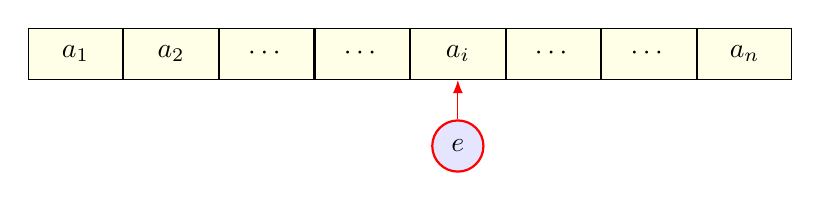
\begin{tikzpicture}[box/.style={draw, minimum width=1.2cm, minimum height=0.65cm, fill=yellow!10}]
	    \draw node[box] (a1) {$a_1$}
	    node[box, right=0 of a1] (a2) {$a_2$}
	    node[box, right=0 of a2] (a3) {$\cdots$}
	    node[box, right=0 of a3] (a4) {$\cdots$}
	    node[box, right=0 of a4] (ai) {$a_i$}
	    node[box, right=0 of ai] (a6) {$\cdots$}
	    node[box, right=0 of a6] (a7) {$\cdots$}
	    node[box, right=0 of a7] (an) {$a_n$}
		  node[draw=red, ellipse, minimum width=0.65cm, minimum height=0.65cm, thick, fill=blue!10, below=0.5 of ai] (cur) {$e$};
		  \draw[draw = red, -Latex] (cur) -- (ai);
    \end{tikzpicture}
  }

  \begin{easylist}
    & 在长为n的线性表中插入一个元素,所需移动元素次数的平均次数为?

    && 有多少种可能的插入位置?$n+1$

    && 假设这些位置以同等概率出现,每个概率$\dfrac{1}{n+1}$。每个情形下分别移动
    $n, n-1, \cdots, 0$次。求加权和为$n/2$。

    && 平均时间复杂度:$T(n)=O(n)$
  \end{easylist}
\end{frame}

\begin{frame}[fragile]
  \frametitle{删除index位置上的元素}
  \scalebox{0.7}{
    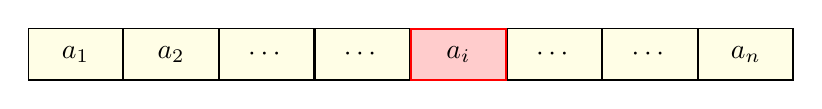
\begin{tikzpicture}[scale=0.5, box/.style={draw, minimum width=1.2cm, minimum height=0.65cm, fill=yellow!10}]
	    \draw node[box] (a1) {$a_1$}
	    node[box, right=0 of a1] (a2) {$a_2$}
	    node[box, right=0 of a2] (a3) {$\cdots$}
	    node[box, right=0 of a3] (a4) {$\cdots$}
	    node[box, draw=red, thick, fill=red!20, right=0 of a4] (ai) {$a_i$}
	    node[box, right=0 of ai] (a6) {$\cdots$}
	    node[box, right=0 of a6] (a7) {$\cdots$}
	    node[box, right=0 of a7] (an) {$a_n$};
    \end{tikzpicture}
  }

  \begin{minted}{java}
boolean remove(int index) {
    if(index<0||index>=length)  
          return false;
    if(getLength()==0)
          return false;
    for (int j=index;j<length-1; j++)    //前移
          Elem[j]=elem[j+1];
    length--;
}
  \end{minted}
\end{frame}

\begin{frame}[fragile]
  \frametitle{删除元素的时间复杂度}
  \scalebox{0.7}{
    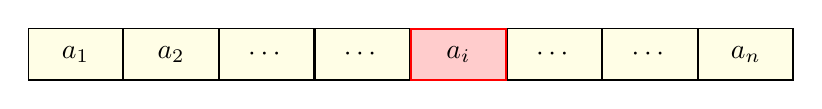
\begin{tikzpicture}[scale=0.5, box/.style={draw, minimum width=1.2cm, minimum height=0.65cm, fill=yellow!10}]
	    \draw node[box] (a1) {$a_1$}
	    node[box, right=0 of a1] (a2) {$a_2$}
	    node[box, right=0 of a2] (a3) {$\cdots$}
	    node[box, right=0 of a3] (a4) {$\cdots$}
	    node[box, draw=red, thick, fill=red!20, right=0 of a4] (ai) {$a_i$}
	    node[box, right=0 of ai] (a6) {$\cdots$}
	    node[box, right=0 of a6] (a7) {$\cdots$}
	    node[box, right=0 of a7] (an) {$a_n$};
    \end{tikzpicture}
  }

  \begin{itemize}
  \item 在长度为n的线性表中删除一个元素:
    \begin{itemize}
    \item 共有n个可能的位置,每个有1/n的概率。每个情形下分别移动n-1, …, 0次。求加权和为(n-1)/2。
    \item $T(n)=O(n)$
    \end{itemize}
  \end{itemize}

  \pause

  \begin{tcolorbox}[standard jigsaw, opacityback=0, colframe=red, title=结论]
    在顺序表中插入或删除一个元素时,平均移动一半元素,当$n$很大时,效率很低.
  \end{tcolorbox}
\end{frame}

\begin{frame}[fragile]
  \frametitle{顺序表特点:地址连续}
  \begin{columns}
    \begin{column}[T]{.5\linewidth}
      \begin{tcolorbox}[]
      \scalebox{0.7}{
        \begin{tikzpicture}[scale=0.5, box/.style={draw, minimum width=1.2cm, minimum height=0.5cm, fill=yellow!10}]
	        \draw node[box] (a1) {$a_1$}
	        node[box, below=0 of a1] (a2) {$a_2$}
	        node[box, below=0 of a2] (a3) {$\cdots$}
	        node[box, below=0 of a3] (ai) {$a_i$}
	        node[box, below=0 of ai] (a5) {$\cdots$}
	        node[box, below=0 of a5] (an) {$a_n$}
	        node[box, below=0 of an, fill=gray!30] (a7) {}
	        node[box, below=0 of a7, fill=gray!30] (a8) {}
	        node[box, below=0 of a8, fill=gray!30] (a9) {};

	        \draw node[right=0.3 of a1] (p1) {$1$}
	        node[right=0.3 of a2] (p2) {$2$}
	        node[right=0.3 of ai] (pi) {$i$}
	        node[right=0.3 of an] (pn) {$n$}
	        node[right=0.3 of a7] (p7) {空闲}
	        node[right=0.3 of a8] (p8) {空闲}
	        node[right=0.3 of a9] (p9) {空闲};

	        \draw node[left=0.3 of a1] (p1) {$b$}
	        node[left=0.3 of a2] (p2) {$b+l$}
	        node[left=0.3 of ai] (pi) {$b+(i-1)\cdot l$}
	        node[left=0.3 of an] (pn) {$b+(n-1)\cdot l$}
	        node[left=0.3 of a7] (p7) {$b+n\cdot l$}
	        node[left=0.3 of a8] (p8) {$\cdots$}
	        node[left=0.3 of a9] (p9) {$b+(MaxLen-1)\cdot l$};
        \end{tikzpicture}
      }
      \end{tcolorbox}
    \end{column}
    \begin{column}[T]{.5\linewidth}
      \begin{easylist}
        & 优点
        && 直观
        && 随机存储效率高
        \pause
        & 缺点
        && 移动元素代价大
      \end{easylist}
    \end{column}
  \end{columns}
\end{frame}


\subsection{链表}
\begin{frame}[fragile]
  \frametitle{方案2: 链式存储---链表}
  \begin{columns}
    \begin{column}[T]{.4\linewidth}
      \scalebox{0.5}{    \begin{tikzpicture}[fill=red, box/.style={draw, minimum width=2cm, minimum height=0.85cm, fill=yellow!10}]
	      \draw node[box] (dh) {数据域}  node[box, right=0 of dh] (ph) {指针域}
	 node[box, below=0.5 of dh] (d_li) {LI}  node[box, right=0 of d_li] (p_li) {43} node[left=0.2 of d_li] {1}
	 node[box, below=0.5 of d_li] (d_qian) {QIAN}  node[box, right=0 of d_qian] (p_qian) {13} node[left=0.2 of d_qian] {7}
	 node[box, below=0.5 of d_qian] (d_sun) {SUN}  node[box, right=0 of d_sun] (p_sun) {1} node[left=0.2 of d_sun] {13}
	 node[box, below=0.5 of d_sun] (d_wang) {WANG}  node[box, right=0 of d_wang] (p_wang) {?} node[left=0.2 of d_wang] {19}
	 node[box, below=0.5 of d_wang] (d_wu) {WU}  node[box, right=0 of d_wu] (p_wu) {37} node[left=0.2 of d_wu] {25}
	 node[box, below=0.5 of d_wu] (d_zhao) {ZHAO}  node[box, right=0 of d_zhao] (p_zhao) {7} node[left=0.2 of d_zhao] {31}
	 node[box, below=0.5 of d_zhao] (d_zheng) {ZHENG}  node[box, right=0 of d_zheng] (p_zheng) {?} node[left=0.2 of d_zheng] {37}
	 node[box, below=0.5 of d_zheng] (d_zhou) {ZHOU}  node[box, right=0 of d_zhou] (p_zhou) {25} node[left=0.2 of d_zhou] {43}
	node[box, minimum width=0.85cm, draw=red, fill=red!20, left=1 of d_li] (h) {31};

	\path[draw=red] (h.center) edge[out=270, in=155, -Latex, draw=red, thick] (d_zhao.west);
	\path[draw=blue] (p_zhao.east) edge[out=0, in=225, -Latex] (d_qian.west);
	\path[draw=blue] (p_qian.east) edge[out=0, in=225, -Latex] (d_sun.west);
	\path[draw=blue] (p_sun.east) edge[out=0, in=225, -Latex] (d_li.west);
\end{tikzpicture}

}
    \end{column}
    \begin{column}[T]{.6\linewidth}
      用一组任意的存储单元存储线性表的数据元素,利用指针指向直接后继的存储位置
    \end{column}
  \end{columns}
\end{frame}

\begin{frame}[fragile]
  \frametitle{单链表的类型定义}
  \begin{columns}
    \begin{column}[T]{.4\linewidth}
      \scalebox{0.5}{    \begin{tikzpicture}[fill=red, box/.style={draw, minimum width=2cm, minimum height=0.85cm, fill=yellow!10}]
	      \draw node[box] (dh) {数据域}  node[box, right=0 of dh] (ph) {指针域}
	 node[box, below=0.5 of dh] (d_li) {LI}  node[box, right=0 of d_li] (p_li) {43} node[left=0.2 of d_li] {1}
	 node[box, below=0.5 of d_li] (d_qian) {QIAN}  node[box, right=0 of d_qian] (p_qian) {13} node[left=0.2 of d_qian] {7}
	 node[box, below=0.5 of d_qian] (d_sun) {SUN}  node[box, right=0 of d_sun] (p_sun) {1} node[left=0.2 of d_sun] {13}
	 node[box, below=0.5 of d_sun] (d_wang) {WANG}  node[box, right=0 of d_wang] (p_wang) {?} node[left=0.2 of d_wang] {19}
	 node[box, below=0.5 of d_wang] (d_wu) {WU}  node[box, right=0 of d_wu] (p_wu) {37} node[left=0.2 of d_wu] {25}
	 node[box, below=0.5 of d_wu] (d_zhao) {ZHAO}  node[box, right=0 of d_zhao] (p_zhao) {7} node[left=0.2 of d_zhao] {31}
	 node[box, below=0.5 of d_zhao] (d_zheng) {ZHENG}  node[box, right=0 of d_zheng] (p_zheng) {?} node[left=0.2 of d_zheng] {37}
	 node[box, below=0.5 of d_zheng] (d_zhou) {ZHOU}  node[box, right=0 of d_zhou] (p_zhou) {25} node[left=0.2 of d_zhou] {43}
	node[box, minimum width=0.85cm, draw=red, fill=red!20, left=1 of d_li] (h) {31};

	\path[draw=red] (h.center) edge[out=270, in=155, -Latex, draw=red, thick] (d_zhao.west);
	\path[draw=blue] (p_zhao.east) edge[out=0, in=225, -Latex] (d_qian.west);
	\path[draw=blue] (p_qian.east) edge[out=0, in=225, -Latex] (d_sun.west);
	\path[draw=blue] (p_sun.east) edge[out=0, in=225, -Latex] (d_li.west);
\end{tikzpicture}

}
    \end{column}
    \begin{column}[T]{.6\linewidth}
      \begin{easylist}
        & 单链表:每个结点有一个指针域
        & 单链表可由头指针唯一确定,头指针指向第一个结点。
        & Java Code:

        \scriptsize

        \begin{minted}{java}
          class Node {
            Object data;
            Node next;
          }
        \end{minted}

      \end{easylist}
    \end{column}
  \end{columns}
\end{frame}

\begin{frame}[fragile]
  \frametitle{单链表的类型定义}
  \begin{columns}
    \begin{column}[T]{.4\linewidth}
      \scalebox{0.5}{    \begin{tikzpicture}[fill=red, box/.style={draw, minimum width=2cm, minimum height=0.85cm, fill=yellow!10}]
	      \draw node[box] (dh) {数据域}  node[box, right=0 of dh] (ph) {指针域}
	 node[box, below=0.5 of dh] (d_li) {LI}  node[box, right=0 of d_li] (p_li) {43} node[left=0.2 of d_li] {1}
	 node[box, below=0.5 of d_li] (d_qian) {QIAN}  node[box, right=0 of d_qian] (p_qian) {13} node[left=0.2 of d_qian] {7}
	 node[box, below=0.5 of d_qian] (d_sun) {SUN}  node[box, right=0 of d_sun] (p_sun) {1} node[left=0.2 of d_sun] {13}
	 node[box, below=0.5 of d_sun] (d_wang) {WANG}  node[box, right=0 of d_wang] (p_wang) {?} node[left=0.2 of d_wang] {19}
	 node[box, below=0.5 of d_wang] (d_wu) {WU}  node[box, right=0 of d_wu] (p_wu) {37} node[left=0.2 of d_wu] {25}
	 node[box, below=0.5 of d_wu] (d_zhao) {ZHAO}  node[box, right=0 of d_zhao] (p_zhao) {7} node[left=0.2 of d_zhao] {31}
	 node[box, below=0.5 of d_zhao] (d_zheng) {ZHENG}  node[box, right=0 of d_zheng] (p_zheng) {?} node[left=0.2 of d_zheng] {37}
	 node[box, below=0.5 of d_zheng] (d_zhou) {ZHOU}  node[box, right=0 of d_zhou] (p_zhou) {25} node[left=0.2 of d_zhou] {43}
	node[box, minimum width=0.85cm, draw=red, fill=red!20, left=1 of d_li] (h) {31};

	\path[draw=red] (h.center) edge[out=270, in=155, -Latex, draw=red, thick] (d_zhao.west);
	\path[draw=blue] (p_zhao.east) edge[out=0, in=225, -Latex] (d_qian.west);
	\path[draw=blue] (p_qian.east) edge[out=0, in=225, -Latex] (d_sun.west);
	\path[draw=blue] (p_sun.east) edge[out=0, in=225, -Latex] (d_li.west);
\end{tikzpicture}

}
    \end{column}
    \begin{column}[T]{.6\linewidth}
      \begin{easylist}
        & 单链表:每个结点有一个指针域
        & 单链表可由头指针唯一确定,头指针指向第一个结点。
        & Python Code:
        \scriptsize

        \begin{minted}{python}
          class Node:
            def __init__(self, data, next=None):
              self.data = data
              self.next = next

          first = Node(1)
          second = Node(2)
          last = Node(3)
          first.next=second
          second.next = last
          print(first.next.next.data)
        \end{minted}

      \end{easylist}
    \end{column}
  \end{columns}
\end{frame}

\begin{frame}[fragile]
  \frametitle{单链表上的常见操作}
  \begin{enumerate}
  \item 建立单链表create()
  \item 求表长length()
  \item 查找index(value)
  \item 插入insert(i,e)
  \item 删除remove(i)
  \item 获取元素get(index)
  \item 显示display()
  \end{enumerate}
\end{frame}

\begin{frame}[fragile]
  \frametitle{建立单链表}
  \begin{itemize}
  \item 链表是{\color{red}动态管理}的:链表中的每个结点占用的存储空间不是预先分
    配,而是运行时系统根据需求而生成的。
  \item 建立单链表从空表开始,每读入一个数据元素则申请一个结点,插入链表。
  \end{itemize}
\end{frame}

\begin{frame}[fragile]
  \frametitle{建立单链表:两种不同方式}
  如依次读入  25, 45, 18…

  \begin{columns}
    \begin{column}[T]{.5\linewidth}
      头部插入:

      \begin{tcolorbox}[]
        \scalebox{0.5}{
          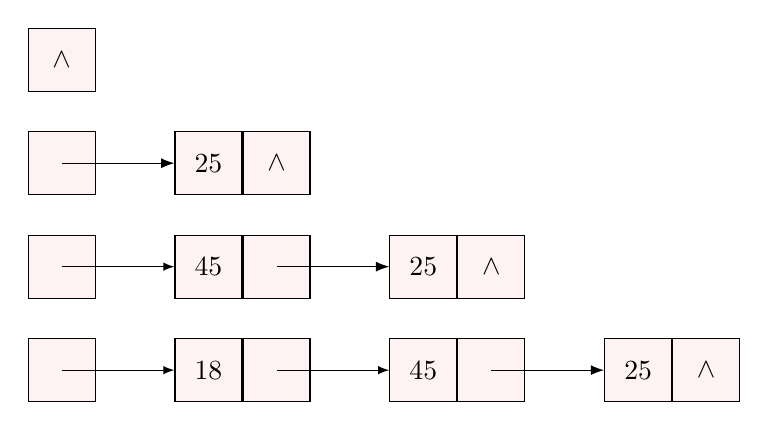
\begin{tikzpicture}[fill=red, box/.style={draw, minimum width=0.85cm, minimum height=0.8cm, fill=red!5}]
	          \draw node[box] (h) {$\wedge$};

	          \draw node[box, below=0.5 of h] (h) {} node[box, right=of h] (d25) {25}  node[box, right=0 of d25] (p25) {$\wedge$};
	          \draw[draw, -Latex] (h.center) -- (d25);

	          \draw node[box, below=0.5 of h] (h) {}
            node[box, right=of h] (d45) {45}  node[box, right=0 of d45] (p45) {}
            node[box, right=of p45] (d25) {25}  node[box, right=0 of d25] (p25) {$\wedge$};
	          \draw[draw, -Latex] (h.center)  edge[-latex] (d45) (p45.center) -- (d25);

	          \draw node[box, below=0.5 of h] (h) {}
            node[box, right=of h] (d18) {18}  node[box, right=0 of d18] (p18) {}
            node[box, right=of p18] (d45) {45}  node[box, right=0 of d45] (p45) {}
            node[box, right=of p45] (d25) {25}  node[box, right=0 of d25] (p25) {$\wedge$};
	          \path[draw, -Latex] (h.center) edge[-latex] (d18) (p18.center)  edge[-latex] (d45)  (p45.center) -- (d25);
          \end{tikzpicture}
        }
      \end{tcolorbox}

    \end{column}
    \begin{column}[T]{.5\linewidth}
      尾部插入:

      \input{figs/list/tail_insert}
    \end{column}
  \end{columns}
\end{frame}

\begin{frame}[fragile]
  \frametitle{建立单链表:头部插入}

  \begin{center}
    \begin{tcolorbox}[]
        \scalebox{0.5}{
          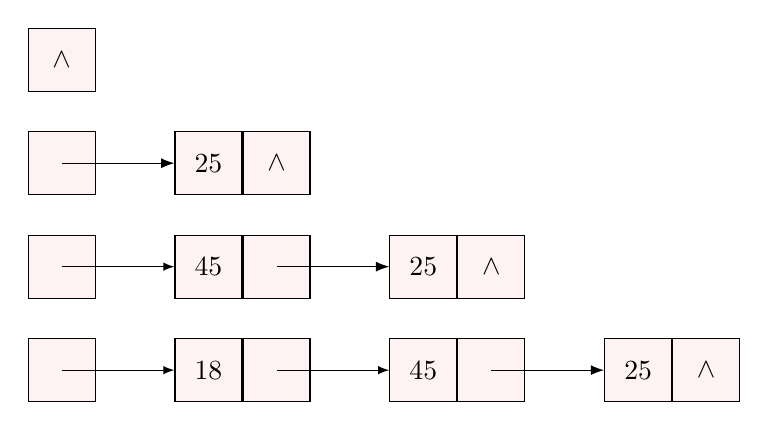
\begin{tikzpicture}[fill=red, box/.style={draw, minimum width=0.85cm, minimum height=0.8cm, fill=red!5}]
	          \draw node[box] (h) {$\wedge$};

	          \draw node[box, below=0.5 of h] (h) {} node[box, right=of h] (d25) {25}  node[box, right=0 of d25] (p25) {$\wedge$};
	          \draw[draw, -Latex] (h.center) -- (d25);

	          \draw node[box, below=0.5 of h] (h) {}
            node[box, right=of h] (d45) {45}  node[box, right=0 of d45] (p45) {}
            node[box, right=of p45] (d25) {25}  node[box, right=0 of d25] (p25) {$\wedge$};
	          \draw[draw, -Latex] (h.center)  edge[-latex] (d45) (p45.center) -- (d25);

	          \draw node[box, below=0.5 of h] (h) {}
            node[box, right=of h] (d18) {18}  node[box, right=0 of d18] (p18) {}
            node[box, right=of p18] (d45) {45}  node[box, right=0 of d45] (p45) {}
            node[box, right=of p45] (d25) {25}  node[box, right=0 of d25] (p25) {$\wedge$};
	          \path[draw, -Latex] (h.center) edge[-latex] (d18) (p18.center)  edge[-latex] (d45)  (p45.center) -- (d25);
          \end{tikzpicture}
        }
      \end{tcolorbox}

  \end{center}

  \begin{minted}[]{java}
Node s = new Node(val);//s指向新结点
s.next = head;//新结点后继为当前头结点
head = s;//头指针指向新结点
  \end{minted}

  \pause
  \color{red} 在空表时是否可行?
\end{frame}


\begin{frame}[fragile]
  \frametitle{建立单链表:尾部插入}

  \begin{center}
    \input{figs/list/tail_insert}
  \end{center}

  \begin{minted}[]{java}
Node s=new Node(val);//s指向新结点
Node r=Findlast(Head);//找到尾结点
r.next=s;//新结点成为尾结点的后继
r=s;
  \end{minted}

  \pause
  \color{red} 在空表时是否可行?
\end{frame}


\begin{frame}[fragile]
  \frametitle{建立单链表:尾部插入}
  \begin{center}
    \input{figs/list/tail_insert}
  \end{center}

  \begin{minted}[]{java}
Node s=new Node(val);
if(!head)  // 空表,插入第一个结点
    head=s; //新结点作为第一个结点
else // 非空表
    r.next=s;//新结点作为最后一个结点的后继

r=s; // 尾指针r 指向新的尾结点
  \end{minted}
\end{frame}

\begin{frame}[fragile]
  \frametitle{头结点问题}
  \begin{easylist}
    & 在上面的算法中,空表和非空表的处理是不同的

    && 当链表为空,新结点作为第一个结点,地址放在链表头指针变量中(第一个结点没
      有前驱,其地址就是整个链表的地址);

    && 否则,新结点地址放在其前驱的指针域。

    & 上述问题在很多操作中都会遇到,为方便操作,可在链表头部加一个“头结点”。
  \end{easylist}

\end{frame}

\begin{frame}[fragile]
  \frametitle{头结点问题}
  \begin{easylist}
    & 头结点的类型与数据结点一致,其数据域无定义,指针域中存放的是第一个数据结点
    的地址,空表时为空。头结点的数据域可以为空,也可存放线性表长度等附加信息,但
    此结点不能计入链表长度值。

    & 加入头结点完全是为了运算的方便。有了头结点,即使是空表,头指针变量head(或
      记作h,或者hp: head pointer)也不为空,空表和“非空表”的处理成为一致。

    & 注意区分:头节点和指向头节点的指针
  \end{easylist}

  \includegraphics[width=0.8\textwidth]{figs/list/header_node_1.png}
\end{frame}

\begin{frame}[fragile]
  \frametitle{求表长}
  \begin{center}
    \scalebox{0.65}{
      \begin{tikzpicture}[fill=red, box/.style={draw, minimum width=0.85cm, minimum height=0.8cm, fill=red!5}]
	      \draw node[box, dashed] (h) {$hp$}
        node[box, thick, double, pattern=north west lines, right=of h] (d18) { }  node[box, thick, double, right=0 of d18] (p18) {}
        node[box, right=of p18] (d45) {45}  node[box, right=0 of d45] (p45) {}
        node[box, right=of p45] (d25) {25}  node[box, right=0 of d25] (p25) {$\wedge$}
	      node[below=1 of h] (tip1) {指向头节点的指针} node[below=1.5 of p18] (tip2) {头节点};
	      \path[draw, -Latex] (h) edge[-latex] (d18) (p18.center)  edge[-latex] (d45)  (p45.center) -- (d25);
	      \path (tip1) edge[draw=red,  thick, ->, out=45, in=270] (h) (tip2) edge[draw=red, thick, in=270, ->] (d18);
      \end{tikzpicture}
    }
  \end{center}

  \scriptsize
  \begin{columns}
    \begin{column}[T]{0.5\linewidth}
      \begin{minted}{c}
        int GetLength() {
          Node p= hp.next; // hp: head pointer
          int  len=0;
          while (p){
            p=p.next;
            len++;
          }
          return  len;
        }
      \end{minted}
    \end{column}
    \begin{column}[T]{0.5\linewidth}
      \pause
      \begin{minted}{python}
class Node:
    def __init__(self, data, next=None):
        self.data = data
        self.next = next

def get_length(hp):
    p = hp.next
    len = 0
    while(p!=None):
        p = p.next
        len = len + 1
    return len

hp = Node(None, Node(45, Node(25)))
print(get_length(hp))
      \end{minted}
    \end{column}
  \end{columns}
\end{frame}

\begin{frame}[fragile]
  \frametitle{单链表的查找}
  \begin{center}
    \scalebox{0.65}{
      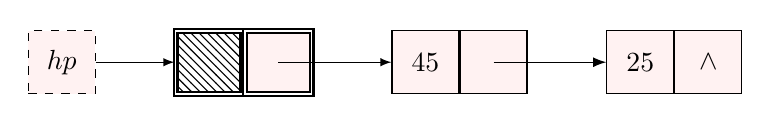
\begin{tikzpicture}[fill=red, box/.style={draw, minimum width=0.85cm, minimum height=0.8cm, fill=red!5}]
	      \draw node[box, dashed] (h) {$hp$}
        node[box, thick, double, pattern=north west lines, right=of h] (d18) { }  node[box, thick, double, right=0 of d18] (p18) {}
        node[box, right=of p18] (d45) {45}  node[box, right=0 of d45] (p45) {}
        node[box, right=of p45] (d25) {25}  node[box, right=0 of d25] (p25) {$\wedge$};
	      \path[draw, -Latex] (h) edge[-latex] (d18) (p18.center)  edge[-latex] (d45)  (p45.center) -- (d25);
      \end{tikzpicture}
    }
  \end{center}

  \begin{itemize}
  \item 按值查找index(value): 是否存在数据元素X?序号是?
  \item 算法思路:“顺藤摸瓜”——从第一个结点开始,判断当前结点的值是否等于x,若是
    则返回该结点的指针,否则继续检查下一个,直到表尾。如果找不到则返回空。
  \end{itemize}

  \begin{minted}{c}
public int index(value){   //在L中查找值为x的结点
  Node  p=hp.next;  int j=0;
  while ( p && p.data !=value){
    p=p->next; j++;
  }
  if(p) return j; else return -1;
}
  \end{minted}
\end{frame}

\begin{frame}[fragile]
  \frametitle{插入新结点:在给定结点的前后}
  \begin{itemize}
  \item 新结点插入到p的后面
    \scalebox{0.65}{
      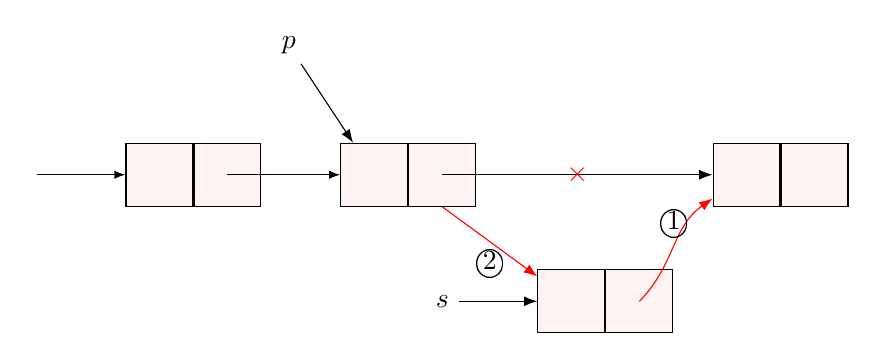
\begin{tikzpicture}[fill=red, box/.style={draw, minimum width=0.85cm, minimum height=0.8cm, fill=red!5}]
        \draw node[] (h) {}
        node[box, right=of h] (d1) { }  node[box, right=0 of d1] (p1) { ~ }
        node[box, right=of p1] (d2) {}  node[box, right=0 of d2] (p2) { ~ }
        node[box, right=3cm of p2] (d3) {}  node[box, right=0 of d3] (p3) {};

        \path[] (h.center) edge[-latex] (d1) (p1.center) edge[-latex] (d2) (p2.center) edge[draw, -Latex] node[color=red] {$\times$} (d3);

        \draw node[above right=of d1](p) {$p$};
        \draw[draw, -Latex] (p) --(d2);

        \draw node[below=of p2] (s) {$s$}
        node[box, right=of s] (ds) { }  node[box, right=0 of ds] (ps) { ~ };
        \draw[draw, -Latex] (s) --(ds);

        \path[] (p2.south) edge[draw=red, -Latex] node[below, align=center] {\textcircled{2}} (ds);
        \path[] (ps.center) edge[draw=red, -Latex, in=215] node[above, align=center] {\textcircled{1}} (d3);
      \end{tikzpicture}
    }

    \begin{minted}{c}
      s.next = p.next;
      p.next = s;
    \end{minted}

  \end{itemize}
\end{frame}

\begin{frame}[fragile]
  \frametitle{插入新结点:在给定结点的前后}
  \begin{itemize}
  \item 新结点插入到p的前面
    \scalebox{0.65}{
      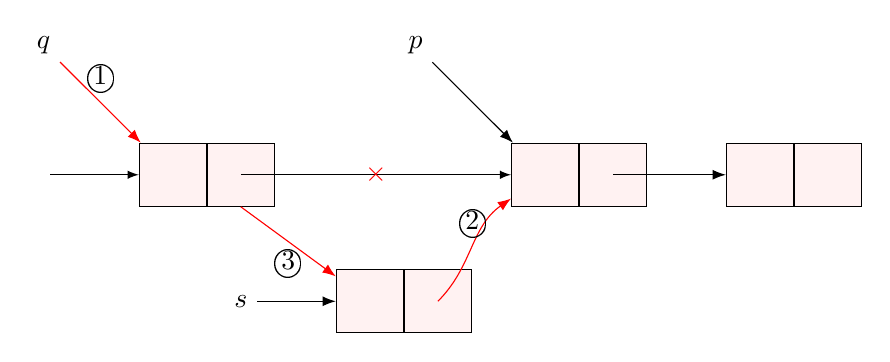
\begin{tikzpicture}[fill=red, box/.style={draw, minimum width=0.85cm, minimum height=0.8cm, fill=red!5}]
        \draw node[] (h) {}
        node[box, right=of h] (d1) { }  node[box, right=0 of d1] (p1) { ~ }
        node[box, right=3cm of p1] (d2) {}  node[box, right=0 of d2] (p2) { ~ }
        node[box, right=of p2] (d3) {}  node[box, right=0 of d3] (p3) {};

        \path[] (h.center) edge[-latex] (d1) (p1.center) edge[-latex] node[color=red] {$\times$} (d2) (p2.center) edge[draw, -Latex]  (d3);

        \draw node[above left=of d2](p) {$p$};
        \draw[draw, -Latex] (p) --(d2);

        \draw node[above left=of d1](q) {$q$};
        \path (q)  edge[draw=red, -Latex] node[above] {\textcircled{1}} (d1);

        \draw node[below=of p1] (s) {$s$}
        node[box, right=of s] (ds) { }  node[box, right=0 of ds] (ps) { ~ };
        \draw[draw, -Latex] (s) --(ds);

        \path[] (p1.south) edge[draw=red, -Latex] node[below, align=center] {\textcircled{3}} (ds);
        \path[] (ps.center) edge[draw=red, -Latex, in=215] node[above, align=center] {\textcircled{2}} (d2);
      \end{tikzpicture}
    }

    找到p的前驱q,在q之后插入s。

    \begin{minted}{c}
q=head;
while (q.next!=p) q=q.next;
s.next=q.next;
q.next=s;
    \end{minted}
  \end{itemize}
\end{frame}

\begin{frame}[fragile]
  \frametitle{插入新结点}
  \begin{easylist}
    & 时间复杂度
    && 后插操作为$O(1)$: 不受$n$的影响
    && 前插操作因为要先找到$p$的前驱,时间性能为$O(n)$。

    \pause
    & 一个小技巧:
    && 将$s$插入到 $p$ 的后面,然后把$p.data$与$s.data$交换,这样能使得时间复杂性为$O(1)$。
  \end{easylist}
\end{frame}

\begin{frame}[fragile]
  \frametitle{删除结点}
  \begin{itemize}
  \item 删除p指向的结点 \\

    \scalebox{0.6}{
      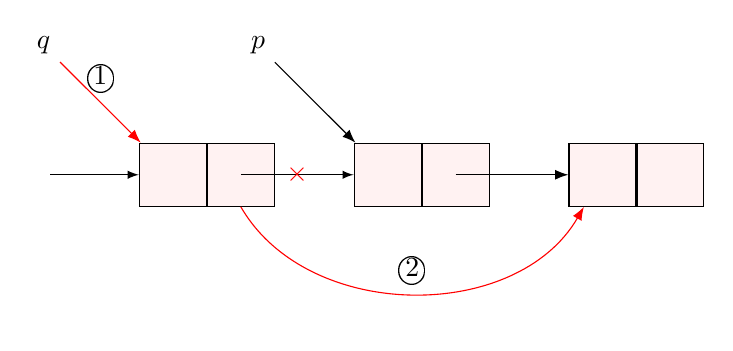
\begin{tikzpicture}[fill=red, box/.style={draw, minimum width=0.85cm, minimum height=0.8cm, fill=red!5}]
        \draw node[] (h) {}
        node[box, right=of h] (d1) { }  node[box, right=0 of d1] (p1) { ~ }
        node[box, right=of p1] (d2) {}  node[box, right=0 of d2] (p2) { ~ }
        node[box, right=of p2] (d3) {}  node[box, right=0 of d3] (p3) {};

        \path[] (h.center) edge[-latex] (d1) (p1.center) edge[-latex] node[color=red] {$\times$} (d2) (p2.center) edge[draw, -Latex]  (d3);

        \draw node[above left=of d2](p) {$p$};
        \draw[draw, -Latex] (p) --(d2);

        \draw node[above left=of d1](q) {$q$};
        \path (q)  edge[draw=red, -Latex] node[above] {\textcircled{1}} (d1);

        \path (p1.south)  edge[draw=red, -Latex, in=240, out=300] node[above]{\textcircled{2}} (d3);
      \end{tikzpicture}
    }

    q.next=q.next.next;
  \item 首先要找到$p$的前驱结点$q$,其时间复杂性为$O(n)$。

  \item 若要删除$p$的后继结点(假设存在),则可以直接完成:\\
    p.next=p.next.next;
  \item 该操作的时间复杂性为$O(1)$ 。
  \end{itemize}
\end{frame}

\begin{frame}[fragile]
  \frametitle{删除第i个结点}
  \begin{minted}{c}
    int  Del(LinkList  L, int i)  //删除链表L第i个结点
    {
      p=get(L, i-1);  //查找第i-1个结点
      if (p==NULL) {
        printf("第i-1个结点不存在");   return -1;
      } else{
        if (!p->next)
          return 0; //第i个结点不存在
        else {
          p.next=p.next.next; //从链表中删除i
          return 1;
        }
      }
    }
  \end{minted}

  算法时间复杂度是$O(n)$
\end{frame}

\begin{frame}[fragile]
  \frametitle{单链表操作小结}
  \begin{itemize}
  \item 在单链表上当前结点之前插入、删除一个结点,必须知道其前驱结点。
  \item 单链表不具有按序号随机访问的特点,只能从头指针开始一个个顺序进行。
  \end{itemize}
\end{frame}

\begin{frame}[fragile]
  \frametitle{单循环链表}
  \begin{easylist}
    & 链表头尾结点相连

    \begin{center}
      \scalebox{0.65}{
        \begin{tikzpicture}[fill=red, box/.style={draw, minimum width=0.85cm, minimum height=0.8cm, fill=red!5}]
	        \draw node[box, dashed] (hp) {$hp$}
          node[box, thick, double, pattern=north west lines, right=of hp] (dh) { }  node[box, thick, double, right=0 of dh] (ph) {}
          node[box, right=of ph] (da1) {$a_1$}  node[box, right=0 of da1] (pa1) {}
          node[box, draw=none, right=of pa1] (dai) {$\cdots$}  node[box, draw=none,  right=0 of dai] (pai) {$\cdots$}
          node[box, right=of pai] (dan) {$a_n$}  node[box, right=0 of dan] (pan) {};

	        \path[draw, -Latex] (hp) edge[-latex] (dh) (ph.center)  edge[-Latex] (da1)
			    (pa1.center) edge[-Latex] (dai)
			    (pai.east) edge[-Latex] (dan)
			    (pan.center)  |- ++(0,-1) -| (dh);

          \draw node[box, dashed, right=1cm of pan] (hp) {$hp$}
          node[box, thick, double, pattern=north west lines, right=of hp] (dh) { }  node[box, thick, double, right=0 of dh] (ph) {};

          \path[draw, -Latex] (hp) edge[-latex] (dh) (ph.center)
			    (ph.center)  |- ++(0,-1) -| (dh);

          \draw node[below=1cm of pa1] {(a) 非空表} node[below=1cm of dh] {(b) 空表};
        \end{tikzpicture}
      }
    \end{center}

    & 结点的定义有什么变化?

    & 链表操作有什么变化?比如:

    && 原来用头结点的next是否为NULL (None)判断空表,现在呢?

    && 原来用结点的next是否为NULL (None)判断尾结点,现在呢?
  \end{easylist}
\end{frame}

\begin{frame}[fragile]
  \frametitle{双向链表}

  \begin{center}
    \scalebox{0.5}{
      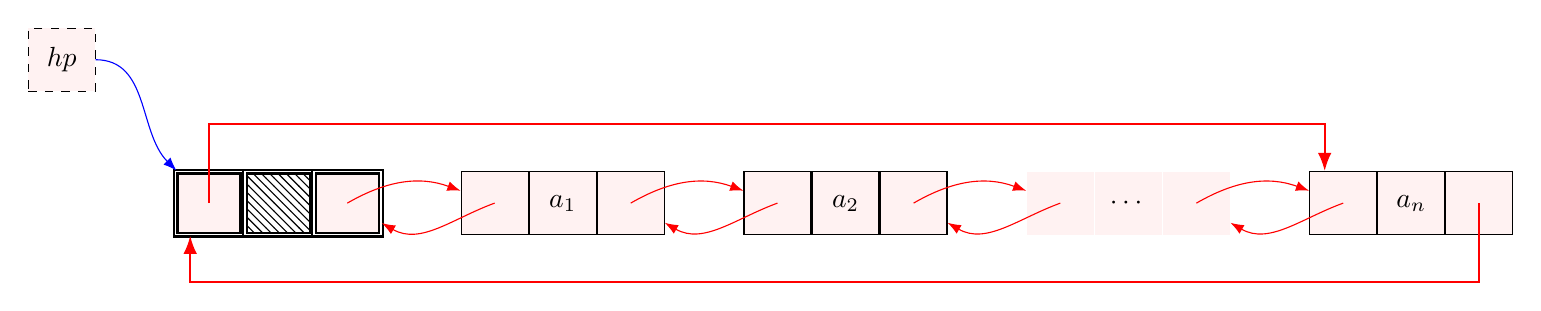
\begin{tikzpicture}[fill=red, box/.style={draw, minimum width=0.85cm, minimum height=0.8cm, fill=red!5},
          e1/.style={draw=red, -Latex, in=160, out=30},
          e2/.style={draw=red, -Latex, in=-30, out=200}
        ]
	      \draw node[box, dashed] (hp) {$hp$}
		    node[box, thick, double,below right=of hp] (prevh) { }
        node[box, thick, double, pattern=north west lines, right=0 of prevh] (datah) { }  node[box, thick, double, right=0 of datah] (nexth) {}

		    node[box, right=of nexth] (prev1) {}   node[box, right=0 of prev1] (data1) {$a_1$}  node[box, right=0 of data1] (next1) {}

		    node[box, right=of next1] (prev2) {}   node[box, right=0 of prev2] (data2) {$a_2$}  node[box, right=0 of data2] (next2) {}

		    node[box, right=of next2, draw=none] (previ) {}   node[box, right=0 of previ, draw=none] (datai) {$\cdots$}  node[box, right=0 of datai, draw=none] (nexti) {}

		    node[box, right=of nexti] (prevn) {}   node[box, right=0 of prevn] (datan) {$a_n$}  node[box, right=0 of datan] (nextn) {};

        \path (hp) edge[out=0, -Latex, draw=blue] (prevh)
	      (nexth.center) edge[e1] (prev1)
        (next1.center) edge[e1] (prev2)
        (next2.center) edge[e1] (previ)
        (nexti.center) edge[e1] (prevn)
	      (prev1.center) edge[e2] (nexth)
        (prev2.center) edge[e2] (next1)
        (previ.center) edge[e2] (next2)
        (prevn.center) edge[e2] (nexti);

        \path[draw=red, thick, -Latex]  (nextn.center)  |- ++(0,-1) -| (prevh.240);
        \path[draw=red, thick, -Latex]  (prevh.center)  |- ++(0,1) -| (prevn.120);
      \end{tikzpicture}
    }

    \scriptsize (a) 有多个节点时的双向链表
  \end{center}

  \begin{columns}
    \begin{column}[T]{0.65\linewidth}
      \scriptsize
      \begin{itemize}
      \item 为什么需要双向链表?
      \item 在单链表中查找后继的时间性能是$O(1)$,查找前驱的时间性能是$O(n)$,如果也
        希望找前驱的时间性能达到$O(1)$,则需要在空间上付出代价 —— 每个结点再加一个指
        向前驱的指针域。
      \item 结点的定义和链表的操作有什么变化?

        \begin{minted}{java}
          class Node {
            Object data;
            Node prior, next;
          }
        \end{minted}
      \end{itemize}
    \end{column}
    \begin{column}[T]{0.35\linewidth}
      \begin{center}
        \scalebox{0.5}{
          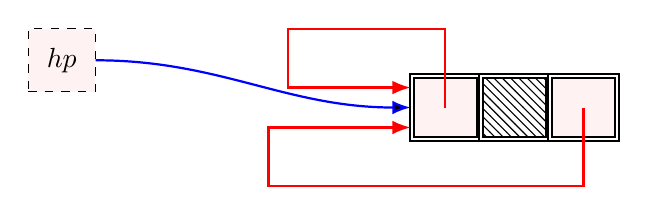
\begin{tikzpicture}[fill=red, box/.style={draw, minimum width=0.85cm, minimum height=0.8cm, fill=red!5},
              e1/.style={draw=red, -Latex, in=160, out=30},
              e2/.style={draw=red, -Latex, in=-30, out=200}
            ]
	          \draw node[box, dashed] (hp) {$hp$}
		        node[box, thick, double, right=4cm of hp, yshift=-0.6cm] (prevh) { }
            node[box, thick, double, pattern=north west lines, right=0 of prevh] (datah) { }  node[box, thick, double, right=0 of datah] (nexth) {};

            \path[draw=blue, thick, -Latex]  (hp)  edge[out=0, in=180] (prevh.180);
            \path[draw=red, thick, -Latex]  (nexth.center)  |- ++(0,-1) -- ++(-4,0) |- (prevh.210);
            \path[draw=red, thick, -Latex]  (prevh.center)  |- ++(0,1) -- ++(-2,0)  |- (prevh.150);
          \end{tikzpicture}
        }

      \scriptsize (b) 只有头节点的情况
      \end{center}
    \end{column}
  \end{columns}
\end{frame}

\begin{frame}[fragile]
  \frametitle{链表特点}
  \begin{center}
    \scalebox{0.65}{
      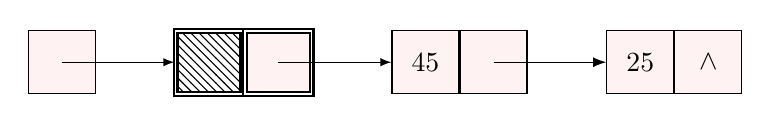
\begin{tikzpicture}[fill=red, box/.style={draw, minimum width=0.85cm, minimum height=0.8cm, fill=red!5}]
	      \draw node[box] (h) {}
        node[box, thick, double, pattern=north west lines, right=of h] (d18) { }  node[box, thick, double, right=0 of d18] (p18) {}
        node[box, right=of p18] (d45) {45}  node[box, right=0 of d45] (p45) {}
        node[box, right=of p45] (d25) {25}  node[box, right=0 of d25] (p25) {$\wedge$};
	      \path[draw, -Latex] (h.center) edge[-latex] (d18) (p18.center)  edge[-latex] (d45)  (p45.center) -- (d25);
      \end{tikzpicture}
    }
  \end{center}

  \begin{easylist}
    & 优点

    && 插入删除方便

    && 动态分配

    \pause

    & 缺点

    && 随机访问效率低
  \end{easylist}
\end{frame}

\begin{frame}[fragile]
  \frametitle{顺序表 VS 链表}
  \begin{columns}
    \begin{column}[T]{0.5\linewidth}
      \begin{tcolorbox}[colframe=red, title=顺序表优点]
        \begin{itemize}
        \item 直观
        \item 随机访问效率高
        \item 没有为表达结点间的逻辑关系增加的额外开销
        \end{itemize}
      \end{tcolorbox}

      \begin{tcolorbox}[colframe=red, title=顺序表缺点]
        \begin{itemize}
        \item 插入删除时效率低
        \item 需要预先分配足够大的存储空间
        \end{itemize}
      \end{tcolorbox}
    \end{column}
    \begin{column}[T]{0.5\linewidth}
\begin{tcolorbox}[colframe=red, title=链表优点]
        \begin{itemize}
        \item 插入删除方便
        \item 动态分配
        \end{itemize}
      \end{tcolorbox}

      \begin{tcolorbox}[colframe=red, title=链表缺点]
        \begin{itemize}
        \item 为表达结点间的逻辑关系增加“指针域”
        \item 随机访问效率低
        \end{itemize}
      \end{tcolorbox}
    \end{column}
  \end{columns}
\end{frame}

\begin{frame}[fragile, allowframebreaks]
  \frametitle{选取恰当的存储结构}
  \begin{enumerate}
  \item 基于存储的考虑

    \begin{itemize}
    \item 使用顺序表,在程序执行之前要明确规定它的存储规模(对MAXSIZE要有合适的
      设定),过大造成浪费,过小造成溢出。可见对线性表的长度或存储规模难以估计时,
      不宜采用顺序表。
    \item 链表不用事先估计存储规模,但链表的存储密度较低。存储密度是指一个结点中
      数据元素所占的存储单元和整个结点所占的存储单元之比。显然链式存储结构的存储
      密度是小于1的。
    \end{itemize}

   \newpage

 \item 基于运算的考虑
   \begin{itemize}
   \item 在顺序表中按序号访问$a_i$的时间性能时$O(1)$,而链表中按序号访问的时间性
     能$O(n)$,所以如果经常做的运算是按序号访问数据元素,显然顺序表优于链表;
   \item 在顺序表中做插入、删除时平均移动表中一半的元素,如果数据元素的信息量较
     大且表较长,不可忽视这一点;
   \item 在链表中作插入、删除,虽然也要找插入位置,但操作主要是比较操作,从这个
     角度考虑优于顺序表。
   \end{itemize}

   \newpage

 \item 其它
   \begin{itemize}
   \item 顺序表容易实现,任何高级语言中都有数组类型,相对来讲简单直观,也是用户
     考虑的一个因素。
   \end{itemize}
  \end{enumerate}

  总之,两种存储结构各有长短,选择那一种由实际问题中的主要因素决定。通常“较稳定”
  的线性表选择顺序存储,而频繁做插入删除的话宜选择链式存储。
\end{frame}

\begin{frame}[fragile]
  \frametitle{本堂小结}
  \begin{enumerate}
  \item 线性表的概念和两种存储方式.
  \item 顺序线性表的特征、基本操作.
  \item 链表的特征、基本操作.
  \item 循环链表和双向链表
  \item 顺序表与链表大PK
  \item 顺序表和链表适用的场合
  \end{enumerate}
\end{frame}

\subsection{作业}
\begin{frame}[fragile]
  \frametitle{约瑟夫环}

  在罗马人占领乔塔帕特后,约瑟夫(Joseph)及他的40个战友躲到一个洞中,这些犹太人
  宁死也不想被敌人抓到,于是决定了一个自杀方式:

  \begin{itemize}
    \item 41个人排成一个圆圈,由第1个人开始报数,每报数到第3人该人就必须自杀,然
      后再由下一个重新报数,直到所有人都自杀身亡为止。
  \item 约瑟夫说他和另一个人逃过了这场死亡游戏: by luck or by the hand of God.
  \item 请问约瑟夫在这个圆圈中的位置是?
  \end{itemize}
\end{frame}

\begin{frame}[fragile]
  \frametitle{约瑟夫环}

  \begin{itemize}
  \item 已知$n$个人 (以编号$1, 2, 3 \cdots n$ 分别表示) 围坐在一张圆桌周围。从
    编号为$k$ 的人开始报数,数到$m$的那个人出列;他的下一个人又从1 开始报数,数
    到$m$的那个人又出列;依此规律重复下去,直到圆桌周围的人全部出列。

  \item 例如:n = 9, k = 1, m = 5;出局顺序如下

  \end{itemize}
  \begin{center}
    \scalebox{0.6} {
      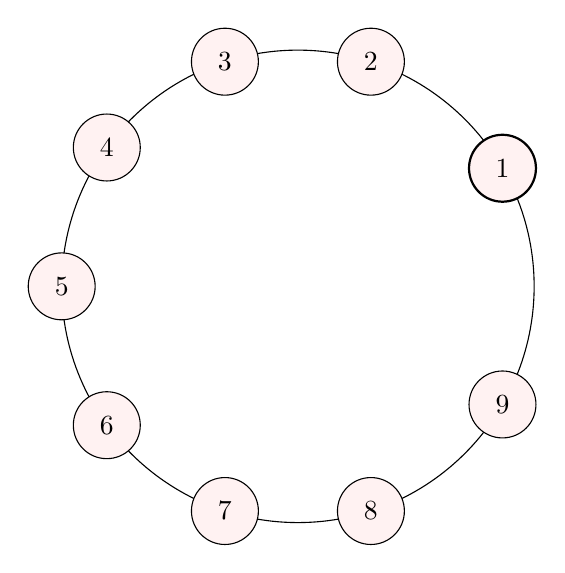
\begin{tikzpicture}[fill=red, ns/.style={draw, circle, minimum width=0.85cm, minimum height=0.8cm, fill=red!5}]
	      \node [draw, minimum size=6cm, circle] {};
        \node (n1) at (30:3cm) [ns, thick]   {1};
        \node (n2) at (72:3cm) [ns]   {2};
        \node (n3) at (108:3cm) [ns]   {3};
        \node (n4) at (144:3cm) [ns]   {4};
        \node (n5) at (180:3cm) [ns]   {5};
        \node (n6) at (216:3cm) [ns]   {6};
        \node (n7) at (252:3cm) [ns]   {7};
        \node (n8) at (288:3cm) [ns]   {8};
        \node (n9) at (330:3cm) [ns]   {9};
      \end{tikzpicture}
    }

    5, 1, 7, 4, 3, 6, 9, 2, 8
  \end{center}
\end{frame}

\begin{frame}[fragile]
  \frametitle{约瑟夫环动画演示}
  见PPT动画
\end{frame}

\section{栈和队列}
\begin{frame}[fragile]
  \frametitle{栈和队列}
  ~
\end{frame}

\subsection{基本概念}
\begin{frame}[fragile]
  \frametitle{栈和队列:两种特殊的线性表}
  \begin{columns}
    \begin{column}[T]{0.5\linewidth}
      \begin{tcolorbox}[colframe=red!80, height=6.5cm, title=栈/Stack]
        \small
        \begin{itemize}
        \item 限制仅在表的一端进行插入和删除。
        \item 通常称插入、删除的一端为栈顶 (Top),另一端为栈底 (Bottom)
        \item LIFO:Last In First Out
        \end{itemize}
      \end{tcolorbox}
    \end{column}
    \begin{column}[T]{0.5\linewidth}
      \begin{tcolorbox}[colframe=blue!80, height=6.5cm, title=队/Queue]
        \small
        \begin{itemize}
        \item 限制仅在表的一端进行插入、在另一端进行删除。
        \item 允许插入的一端称队尾 (rear),允许删除的一段称为队头 (front)。
        \item FIFO:First In First Out
        \end{itemize}
      \end{tcolorbox}
    \end{column}
  \end{columns}
\end{frame}

\begin{frame}[fragile]
  %\frametitle{不同场合下的栈}
  \begin{center}
    \includegraphics[width=0.7\textwidth]{figs/stack/Stack-data-structure.png}
  \end{center}

  \begin{easylist}
    & 操作系统中的栈

    && 由编译器自动分配释放 ,存放函数的参数值,局部变量的值等。栈使用的是一级缓
    存,被调用时处于存储空间中,调用完毕立即释放。

    & 数据结构中的栈

    && 一种后进先出的数据结构
  \end{easylist}
\end{frame}

\begin{frame}[fragile]
  \frametitle{为什么设计栈、研究栈?}
  \scriptsize
  \begin{itemize}
  \item 栈的一个重要应用是在程序设计中实现递归,从而使许多实际问题大大简化。
  \end{itemize}

  \begin{columns}
    \begin{column}[T]{0.5\linewidth}
      \includegraphics[width=0.9\textwidth]{figs/stack/Tower-Of-Hanoi-1.png}
    \end{column}
    \begin{column}[T]{0.5\linewidth}
        \begin{itemize}
        \item 上帝创造世界的时候做了三根金刚石柱子,在一根柱子上从下往上按大小顺
          序摞着64片黄金圆盘。上帝命令婆罗门把圆盘从下面开始按大小顺序重新摆放在
          另一根柱子上,并且规定一次只能移动一个圆盘,在小圆盘上不能放大圆盘。
        \item 有预言说,这件事完成时宇宙会在一瞬间闪电式毁灭。也有人相信婆罗门至
          今还在一刻不停地搬动着圆盘。
        \item \color{red} 18,446,744,073,709,551,615次搬动才能挪完64片金盘!
        \end{itemize}
    \end{column}
  \end{columns}
\end{frame}

\begin{frame}[fragile]
  \frametitle{举例:计算n的阶乘}
  \scriptsize
  \begin{columns}
    \begin{column}[T]{0.4\linewidth}
      \begin{minted}{java}
        int factorial (int n) {
          int  f ;
          if (n==1) f=1;
          else f=n*fact (n-1) ;
          return f;
        }
      \end{minted}
    \end{column}
    \begin{column}[T]{0.6\linewidth}
      \begin{enumerate}
      \item 将调用函数的现场(各寄存器的值,中断时的程序地址等)入栈,转入被调函数;
      \item 执行被调函数,如又调用其它函数,则执行上述步骤;
      \item 被调函数执行完,取栈顶的值,恢复调用函数时的现场,根据现场中的指令地
        址,恢复调用函数在中断处继续执行。
      \end{enumerate}
    \end{column}
  \end{columns}
  \includegraphics[width=0.9\textwidth]{figs/stack/factorial.png}
\end{frame}

\subsection{栈的存储表示方法}
\begin{frame}[fragile]
  \frametitle{栈的存储表示方法}
  \begin{tcolorbox}[colframe=red]
    请考虑其常用操作。试想选用顺序存储还是链式存储?
  \end{tcolorbox}

  \begin{columns}
    \begin{column}[T]{0.1\textwidth}
      \includegraphics[width=1cm]{figs/stack/apple.png}
    \end{column}
    \begin{column}[T]{0.5\textwidth}
      \begin{easylist}
        & 特点:后进先出

        && 1、经常性的在栈顶插入新元素,以及取栈顶元素;

        && 2、无须访问非栈顶元素。
      \end{easylist}
    \end{column}
    \begin{column}[T]{0.4\textwidth}
      \includegraphics[width=3cm]{figs/stack/pushpop.png}
    \end{column}
  \end{columns}
\end{frame}

\begin{frame}[fragile]
  \frametitle{1. 顺序栈}
  \begin{columns}
    \begin{column}[T]{0.5\linewidth}
      \includegraphics[width=0.7\textwidth]{figs/stack/seq-stack.png}
    \end{column}
    \begin{column}[T]{0.5\linewidth}
      \begin{enumerate}
      \item 顺序栈中元素用地址连续的存储单元依次存放;
      \item 栈底位置固定不变;
      \item 栈顶位置top随着进栈和出栈的操作而变化。
      \end{enumerate}

      顺序栈类型定义:

      \begin{minted}{c}
        class stack<Elem>{
          Object[] data;
          int top;
          int maxSize;
        } SeqStack;
      \end{minted}
    \end{column}
  \end{columns}
\end{frame}

\begin{frame}[fragile]
  \begin{easylist}
    & 动态分配
    && 先为栈分配一个初始容量,在栈的空间不够使用时再逐段扩大。

    & 指针base
    && 始终指向栈底位置,如果base为NULL表示栈不存在;

    & 指针top
    && 初值指向栈底,即top = =base,表示栈空;(不唯一)
    && 每当插入新的栈顶元素,指针top++;
    && 每当删除栈顶元素,指针top--;
    && 非空栈中的栈顶指针始终在栈顶元素的下一个位置上。
  \end{easylist}

  \centering
  \includegraphics[width=0.8\textwidth]{figs/stack/stack-demo.png}
\end{frame}

\begin{frame}[fragile]
  \begin{columns}
    \begin{column}[T]{0.5\linewidth}
      \begin{tcolorbox}[height=8cm]
        对于顺序栈,入栈需要判栈是否满,是则需要中止、或重新分配空间,否则出现空间溢出。

        \begin{minted}{java}
public Boolean push (Elem e) {
  if ( top==maxSize) {
    print("栈已满");
    return false;
  }
  data[top++] = e;
  return true;
}
        \end{minted}
      \end{tcolorbox}
    \end{column}
    \begin{column}[T]{0.5\linewidth}
      \pause
      \begin{tcolorbox}[height=8cm]
        出栈首先要判断栈是否为空;否则栈空时进行操作将出现下溢错误。

        \begin{minted}{java}
public Elem pop() {
  if(top==base) {
    return null;
  } else {
    top = top-1
    return data[top];
  }
}
        \end{minted}
      \end{tcolorbox}
    \end{column}
  \end{columns}
\end{frame}


\subsection{链栈}
\begin{frame}[fragile]
  \frametitle{2. 链栈}

  \small

  \begin{columns}
    \begin{column}[T]{0.7\linewidth}
      \begin{easylist}
        & 链栈有无栈满溢出问题?

        & 指针如何指?

        && 从栈顶依次向后指,因为操作主要是在栈顶插入、删除,经常需要根据栈顶元
        素找次顶元素。

        & 是否要加头结点?

        && No. 因为头部插入不会出现处理不一致的问题.
      \end{easylist}

      写出链栈的类型定义:

      \begin{minted}{java}
        class Node{
          Elem data;
          Node next;
        }

        Node  top ; // 链栈
      \end{minted}
    \end{column}
    \begin{column}[T]{0.3\linewidth}
      \scalebox{0.8}{
        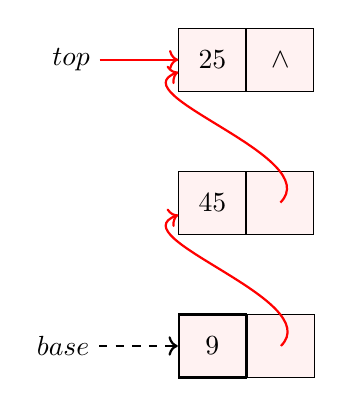
\begin{tikzpicture}[fill=red, box/.style={draw, minimum width=0.85cm, minimum height=0.8cm, fill=red!5}]
	        \draw node[] (base) {$base$}
          node[box, thick, right=of base] (d1) { 9 }   node[box, right=0 of d1] (p1) {}
          node[box, above=of d1] (d2) {45}  node[box, right=0 of d2] (p2) {}
          node[box, above=of d2] (d3) {25}  node[box, right=0 of d3] (p3) {$\wedge$}
	        node[left= of d3] (top) {$top$};

          \path (base) edge[draw, dashed, thick, ->] (d1) (top) edge[draw=red, thick, ->] (d3);
		      \path (p1.center) edge[draw=red,  thick, ->, out=45, in=200] (d2) (p2.center) edge[draw=red, thick, in=200, ->] (d3);
        \end{tikzpicture}
      }
    \end{column}
  \end{columns}
\end{frame}

\begin{frame}[fragile]
% \frametitle{链栈基本操作}

  请尝试写出入栈出栈的算法

  \begin{minted}{java}
    public push (Elem e) {
      //是否还要判断栈是否满?
      top=new Node(e, top);
      return OK;
   }

   public pop( ){
     //是否还要判断栈是否空?
     e=top;
     top=top.next;
     e.next=null;
     return e.data;
}
  \end{minted}

\end{frame}

\begin{frame}[fragile]
  \frametitle{栈的应用}
  迷宫求解(见PPT)
\end{frame}

\section{队列}

\begin{frame}[fragile]
  \frametitle{队/Queue}
   \begin{columns}
    \begin{column}[T]{0.5\linewidth}
      \begin{tcolorbox}[colframe=blue!80, height=6.5cm, title=队/Queue]
        \small
        \begin{itemize}
        \item 限制仅在表的一端进行插入、在另一端进行删除。
        \item 允许插入的一端称队尾 (rear),允许删除的一段称为队头 (front)。
        \item FIFO:First In First Out
        \end{itemize}
      \end{tcolorbox}
    \end{column}
    \begin{column}[T]{0.5\linewidth}
      \includegraphics[width=0.9\textwidth]{figs/queue/queueofpeople.png}

      \begin{itemize}
      \item 比如生活中排队购物、操作系统中的作业排队等。
      \end{itemize}
    \end{column}
  \end{columns}
\end{frame}


\subsection{队的存储表示方法}
\begin{frame}[fragile]
  \frametitle{队的存储表示方法}

  \begin{itemize}
  \item 队也有两种存储表示方法:顺序队、链队
  \item 顺序队:利用地址连续的存储单元依次存放数据元素。
  \end{itemize}

  \begin{columns}
    \begin{column}[T]{0.5\linewidth}
      \scalebox{0.6}{
        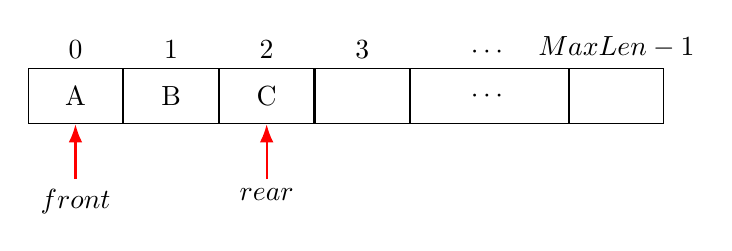
\begin{tikzpicture}[scale=0.5, box/.style={draw, minimum width=1.2cm, minimum height=0.7cm}]
		      \draw node[box] (a0) {A}
	        node[box, right=0 of a0] (a1) {B}
	        node[box, right=0 of a1] (a2) {C}
	        node[box, right=0 of a2] (a3) {}
          node[box, right=0 of a3, minimum width=2cm] (amore) {$\cdots$}
	        node[box, right=0 of amore] (alast) {}
		      node[above=0 of a0] {0}
				  node[above=0 of a1] {1}
				  node[above=0 of a2] {2}
				  node[above=0 of a3] {3}
				  node[above=0 of amore] {$\cdots$}
				  node[above=0 of alast] {$MaxLen-1$}
	        node[below=0.7cm of a0] (front) {$front$}
	        node[below=0.7cm of a2] (rear) {$rear$};

			    \draw[draw=red, thick, -Latex] (front) -> (a0);
          \draw[draw=red, thick, -Latex] (rear) -> (a2);
        \end{tikzpicture}
      }
    \end{column}
    \begin{column}[T]{0.5\linewidth}
      请写出顺序队的类型定义:

      \begin{minted}{java}
        class SeqQueue{
          ElemType  data[ ];
          int maxsize;
          int rear; //队尾,以此计算队长
        }
      \end{minted}

       可否??
    \end{column}
  \end{columns}
\end{frame}

\begin{frame}[fragile]
  \frametitle{顺序队的基本操作}
  \begin{easylist}
    & 入队:如有空间,元素$x$入队后队尾指针加1

    && data[rear++]=x;

    & 出队:如有元素,队头指针加1,表明队头元素出队。

    && x=sq.data[sq.front++];
  \end{easylist}

  \vspace{1cm}

  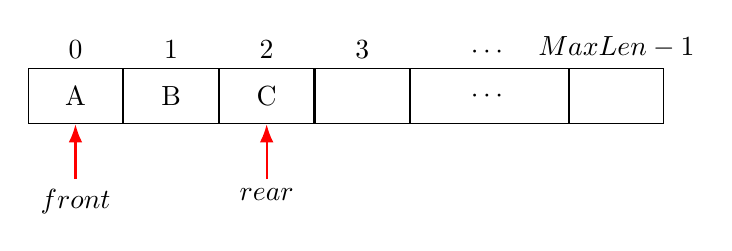
\begin{tikzpicture}[scale=0.5, box/.style={draw, minimum width=1.2cm, minimum height=0.7cm}]
		\draw node[box] (a0) {A}
	  node[box, right=0 of a0] (a1) {B}
	  node[box, right=0 of a1] (a2) {C}
	  node[box, right=0 of a2] (a3) {}
    node[box, right=0 of a3, minimum width=2cm] (amore) {$\cdots$}
	  node[box, right=0 of amore] (alast) {}
		node[above=0 of a0] {0}
		node[above=0 of a1] {1}
		node[above=0 of a2] {2}
		node[above=0 of a3] {3}
		node[above=0 of amore] {$\cdots$}
		node[above=0 of alast] {$MaxLen-1$}
	  node[below=0.7cm of a0] (front) {$front$}
	  node[below=0.7cm of a2] (rear) {$rear$};

		\draw[draw=red, thick, -Latex] (front) -> (a0);
    \draw[draw=red, thick, -Latex] (rear) -> (a2);
  \end{tikzpicture}
\end{frame}

\begin{frame}[fragile]
  \scriptsize
  \begin{itemize}
  \item 设maxsize=10。请你写出如下状态或执行某操作后的顺序队元素。
    \begin{enumerate}
    \item 空队;
    \item a0, a1, a2依次入队;
    \item a3, a4, a5, a6, a7, a8依次入队, a0, a1, a2, a3, a4, a5依次出队;
    \item a9, a10入队。
    \end{enumerate}
  \end{itemize}

  \begin{columns}
    \begin{column}[T]{0.2\linewidth}
      \scalebox{0.8}{
        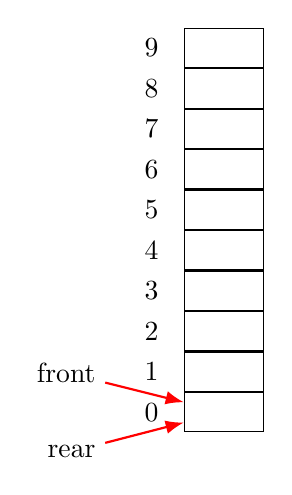
\begin{tikzpicture}[scale=0.5, box/.style={draw, minimum width=1cm, minimum height=0.5cm}]
          \draw node[box] (a0) {} node[left=0.2cm of a0]{0};
          \foreach \i in {1,...,9} {
            \pgfmathtruncatemacro{\x}{\i - 1};
            \draw node[box, above=0 of a\x] (a\i) {} node[left=0.2cm of a\i]{\i};
          }

          \draw node[left=1cm of a0, yshift=0.5cm] (front) {front}  node[left=1cm of a0, yshift=-0.5cm] (rear) {rear};
          \draw[draw=red, thick, -Latex] (front) -> (a0);
          \draw[draw=red, thick, -Latex] (rear) -> (a0);
        \end{tikzpicture}
      }

      (a) 空队
    \end{column}
    \begin{column}[T]{0.2\linewidth}
      \scalebox{0.8}{
        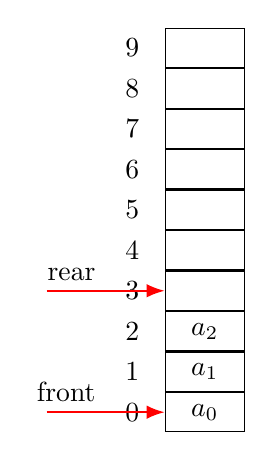
\begin{tikzpicture}[scale=0.5, box/.style={draw, minimum width=1cm, minimum height=0.5cm}]
          \draw node[box] (a0) {$a_0$} node[left=0.2cm of a0]{0};
          \foreach \i in {1,...,2} {
            \pgfmathtruncatemacro{\x}{\i - 1};
            \draw node[box, above=0 of a\x] (a\i) {$a_\i$} node[left=0.2cm of a\i]{\i};
          }
          \foreach \i in {3,...,9} {
            \pgfmathtruncatemacro{\x}{\i - 1};
            \draw node[box, above=0 of a\x] (a\i) {} node[left=0.2cm of a\i]{\i};
          }

          \draw node[left=1.5cm of a0] (front) {}  node[left=1.5cm of a3] (rear) {};
          \path[] (front)  edge[draw=red, thick, -Latex, above left] node{front} (a0);
          \path[] (rear)  edge[draw=red, thick, -Latex, above left] node{rear} (a3);
        \end{tikzpicture}
      }

      (b) 有3个元素
    \end{column}
    \begin{column}[T]{0.2\linewidth}
      \scalebox{0.8}{
        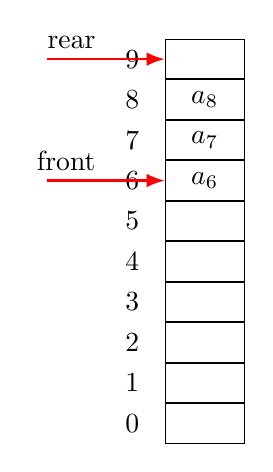
\begin{tikzpicture}[scale=0.5, box/.style={draw, minimum width=1cm, minimum height=0.5cm}]
          \draw node[box] (a0) {} node[left=0.2cm of a0]{0};
          \foreach \i in {1,...,5} {
            \pgfmathtruncatemacro{\x}{\i - 1};
            \draw node[box, above=0 of a\x] (a\i) {} node[left=0.2cm of a\i]{\i};
          }
          \foreach \i in {6,...,8} {
            \pgfmathtruncatemacro{\x}{\i - 1};
            \draw node[box, above=0 of a\x] (a\i) {$a_\i$} node[left=0.2cm of a\i]{\i};
          }
          \foreach \i in {9,...,9} {
            \pgfmathtruncatemacro{\x}{\i - 1};
            \draw node[box, above=0 of a\x] (a\i) {} node[left=0.2cm of a\i]{\i};
          }

          \draw node[left=1.5cm of a6] (front) {}  node[left=1.5cm of a9] (rear) {};
          \path[] (front)  edge[draw=red, thick, -Latex, above left] node{front} (a6);
          \path[] (rear)  edge[draw=red, thick, -Latex, above left] node{rear} (a9);
        \end{tikzpicture}
      }

      (c) 一般情况
    \end{column}
    \begin{column}[T]{0.2\linewidth}
      \scalebox{0.8}{
        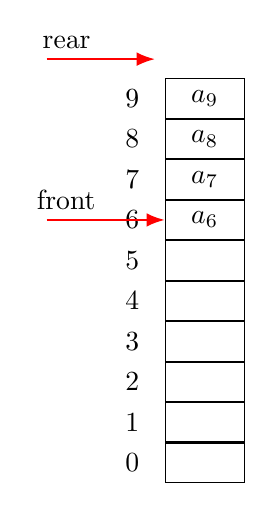
\begin{tikzpicture}[scale=0.5, box/.style={draw, minimum width=1cm, minimum height=0.5cm}]
          \draw node[box] (a0) {} node[left=0.2cm of a0]{0};
          \foreach \i in {1,...,5} {
            \pgfmathtruncatemacro{\x}{\i - 1};
            \draw node[box, above=0 of a\x] (a\i) {} node[left=0.2cm of a\i]{\i};
          }
          \foreach \i in {6,...,9} {
            \pgfmathtruncatemacro{\x}{\i - 1};
            \draw node[box, above=0 of a\x] (a\i) {$a_\i$} node[left=0.2cm of a\i]{\i};
          }

          \draw node[left=1.5cm of a6] (front) {}  node[left=1.5cm of a9, yshift=0.5cm] (rear) {};
          \path[] (front)  edge[draw=red, thick, -Latex, above left] node{front} (a6);
          \path[] (rear)  edge[draw=red, thick, -Latex, above left] node{rear} ++(3,0);
        \end{tikzpicture}
      }

      (d) 假溢出现象
    \end{column}
    \begin{column}[T]{0.2\linewidth}
      \pause
      \begin{itemize}
      \item 入队出队会使整个队列整体后移
      \item “假溢出”: 队尾指针已经移到了最后,不能再执行入队操作,但此时队中并未
        真的“满员” 。如何解决这个问题?
      \end{itemize}
    \end{column}
  \end{columns}
\end{frame}

\begin{frame}[fragile]
  \frametitle{}
  \begin{itemize}
  \item Linear Queue入队出队会使整个队列整体后移
  \item “假溢出”: 队尾指针已经移到了最后,不能再执行入队操作,但此时队中并未
    真的“满员” 。如何解决这个问题?
    \begin{enumerate}
    \item 平移元素;
    \item {\color{red}循环队列 (Circular Queue):将顺序队列的存储区假想为环状空
      间。}在假溢出时,将新元素插入到第一个位置上,这样做,虽物理上队尾在队首之
      前,但逻辑上队首仍然在前。入列和出列仍按“先进先出”的原则进行。

      \begin{itemize}
      \item 入队时的队尾指针操作: \\
        rear=(rear+1) \% maxsize;
      \item 出队时的队头指针操作:\\
		    front=(front+1) \% maxsize;
      \end{itemize}
    \end{enumerate}
  \end{itemize}
\end{frame}

\begin{frame}[fragile]
  \frametitle{循环队列 (Circular Queue)\footnote{延伸阅读:\url{https://en.wikipedia.org/wiki/Circular\_buffer}
  }}
  \small
  \begin{itemize}
  \item head/front points to the first (oldest) used element --- the next element to be read
  \item tail/rear points to the first (oldest) unused element --- the next element to be written
  \item rear: 多数情况下指向尾部元素,tail: 多数情况下指向尾部的下一个元素。教材
    中的rear等同于tail
  \end{itemize}

  \begin{columns}
    \begin{column}[T]{0.5\linewidth}
      \includegraphics[width=0.55\textwidth]{figs/stack/circular-queue-1.png}
    \end{column}
    \begin{column}[T]{0.5\linewidth}
      \includegraphics[width=0.75\textwidth]{figs/stack/circular-queue-2.png}
    \end{column}
  \end{columns}
\end{frame}

\begin{frame}[fragile]
  \begin{easylist}
    & 设maxsize=10。队列状态如(a)所示。请写出分别执行如下操作后的front和rear值:
    && 情况1: a9, a10, a11, a12, a13, a14依次入队
    && 情况2: a5, a6, a7, a8依次出队
  \end{easylist}

  \pause

  \centering
  \begin{columns}
    \begin{column}[T]{0.3\linewidth}
      (a) 有4个元素

      \scalebox{0.8}{
        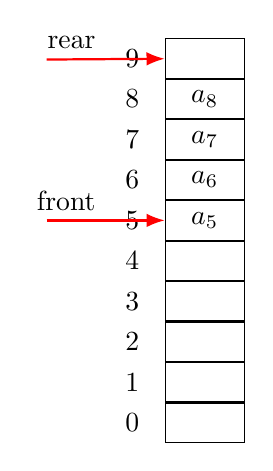
\begin{tikzpicture}[scale=0.5, box/.style={draw, minimum width=1cm, minimum height=0.5cm}]
          \draw node[box] (a0) {} node[left=0.2cm of a0]{0};
          \foreach \i in {1,...,4} {
            \pgfmathtruncatemacro{\x}{\i - 1};
            \draw node[box, above=0 of a\x] (a\i) {} node[left=0.2cm of a\i]{\i};
          }
          \foreach \i in {5,...,8} {
            \pgfmathtruncatemacro{\x}{\i - 1};
            \draw node[box, above=0 of a\x] (a\i) {$a_\i$} node[left=0.2cm of a\i]{\i};
          }
          \foreach \i in {9,...,9} {
            \pgfmathtruncatemacro{\x}{\i - 1};
            \draw node[box, above=0 of a\x] (a\i) {} node[left=0.2cm of a\i]{\i};
          }
          \draw node[left=1.5cm of a5] (front) {}  node[left=1.5cm of a8, yshift=0.5cm] (rear) {};
          \path[] (front)  edge[draw=red, thick, -Latex, above left] node{front} (a5);
          \path[] (rear)  edge[draw=red, thick, -Latex, above left] node{rear}  (a9);
        \end{tikzpicture}
      }
    \end{column}
    \begin{column}[T]{0.4\linewidth}
      (b) 情况1:队满

      \scalebox{0.8}{
        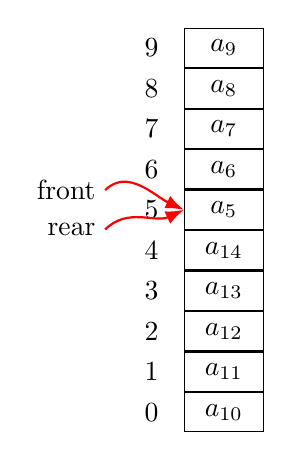
\begin{tikzpicture}[scale=0.5, box/.style={draw, minimum width=1cm, minimum height=0.5cm}]
          \draw node[box] (a0) {$a_{10}$} node[left=0.2cm of a0]{0};
          \foreach \i in {1,...,4} {
            \pgfmathtruncatemacro{\x}{\i - 1};
            \pgfmathtruncatemacro{\v}{\i + 10};
            \draw node[box, above=0 of a\x] (a\i) {$a_{\v}$} node[left=0.2cm of a\i]{\i};
          }
          \foreach \i in {5,...,9} {
            \pgfmathtruncatemacro{\x}{\i - 1};
            \draw node[box, above=0 of a\x] (a\i) {$a_\i$} node[left=0.2cm of a\i]{\i};
          }

          \draw node[left=1cm of a5,yshift=0.25cm] (front) {front}  node[left=1cm of a5,  yshift=-0.25cm] (rear) {rear};
          \path[] (front.east)  edge[draw=red, thick, -Latex,  in=155] node{}  (a5.west);
          \path[] (rear.east)  edge[draw=red, thick, -Latex, in=205] node{}   (a5.west);
        \end{tikzpicture}
      }

    \end{column}
    \begin{column}[T]{0.3\linewidth}
      (c) 情况2:队空

      \scalebox{0.8}{
        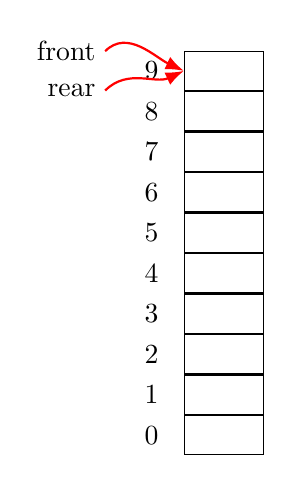
\begin{tikzpicture}[scale=0.5, box/.style={draw, minimum width=1cm, minimum height=0.5cm}]
          \draw node[box] (a0) {} node[left=0.2cm of a0]{0};
          \foreach \i in {1,...,9} {
            \pgfmathtruncatemacro{\x}{\i - 1};
            \draw node[box, above=0 of a\x] (a\i) {} node[left=0.2cm of a\i]{\i};
          }

          \draw node[left=1cm of a9,yshift=0.25cm] (front) {front}  node[left=1cm of a9,  yshift=-0.25cm] (rear) {rear};
          \path[] (front.east)  edge[draw=red, thick, -Latex,  in=155] node{}  (a9.west);
          \path[] (rear.east)  edge[draw=red, thick, -Latex, in=205] node{}   (a9.west);
        \end{tikzpicture}
      }
    \end{column}
  \end{columns}

  当front=rear, 队满还是队空?如何判断队满?如何判断队空?
\end{frame}

\begin{frame}[fragile]
  \frametitle{循环队的队满判别}

  \begin{columns}
    \begin{column}[T]{0.7\linewidth}
      \begin{easylist}
        & 方法一

        && 附设一个存储队中元素个数的变量如num,当num=0时队空,当num=maxsize时为
        队满。

        & 方法二

        && 少用一个元素空间,把右图所示情况视为队满,此时的状态是队尾指针加1就会
        从后面赶上队头指针: (rear+1) \% maxsize==front,从而和空队区别开来。
      \end{easylist}
    \end{column}
    \begin{column}[T]{0.3\linewidth}
      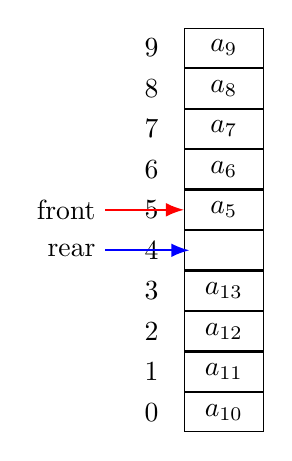
\begin{tikzpicture}[scale=0.5, box/.style={draw, minimum width=1cm, minimum height=0.5cm}]
        \draw node[box] (a0) {$a_{10}$} node[left=0.2cm of a0]{0};
        \foreach \i in {1,...,3} {
          \pgfmathtruncatemacro{\x}{\i - 1};
          \pgfmathtruncatemacro{\v}{\i + 10};
          \draw node[box, above=0 of a\x] (a\i) {$a_{\v}$} node[left=0.2cm of a\i]{\i};
        }
        \draw node[box, above=0 of a3] (a4) {} node[left=0.2cm of a4]{4};
        \foreach \i in {5,...,9} {
          \pgfmathtruncatemacro{\x}{\i - 1};
          \draw node[box, above=0 of a\x] (a\i) {$a_\i$} node[left=0.2cm of a\i]{\i};
        }

        \draw node[left=1cm of a5] (front) {front}  node[left=1cm of a4] (rear) {rear};
        \path[] (front)  edge[draw=red, thick, -Latex, left] node{}  ++ (3,0);
        \path[] (rear)  edge[draw=blue, thick, -Latex, left] node{}   ++ (3,0);
      \end{tikzpicture}
    \end{column}
  \end{columns}
\end{frame}

\begin{frame}[fragile]
  \frametitle{循环队的基本操作}
  \scriptsize
  \begin{minted}{java}
    class SeqQueue  {
      ElemType data[];
      int maxsize;
      int front, rear;  /*队头队尾指针*/
      int num;          /*队中元素的个数*/
    }

    // 入队
    int InQueue (ElemType  x){
      if  (num==maxsize) {
        printf("队满");  return 0;
      } else {
        data[rear]=x;
        rear=(rear+1) % maxsize;
        num++;
        return 1;    /*入队完成*/
      }
    }
  \end{minted}
\end{frame}

\begin{frame}[fragile]
  \frametitle{循环队的基本操作}
  \scriptsize
  \begin{minted}{java}
    //出队
    int OutQueue (ElemType  x) {
      if  (num==0) {
        printf("队空");
        return –1;
      } else {
        x=data[front];  /*读出队头元素*/
        front=(front+1) % maxsize;
        num--;
        return 1;    /*出队完成*/
      }
    }
  \end{minted}
\end{frame}


\begin{frame}[fragile]
  Python:

  \scriptsize
  \begin{minted}{python}
class SeqQueue:
    def __init__(self, max_size=10):
        self.max_size = max_size + 1 # 实际多放一个空间,区分对空、队满
        self.front = 0
        self.rear = 0
        self.elements = [None]*max_size

    def enqueue(self, element) -> bool:
        if (self.rear + 1) % self.max_size == self.front:
            print('Queue is Full!')
            return False
        else:
            self.elements[self.rear] = element
            self.rear = (self.rear + 1) % self.max_size
            return True

    def dequeue(self):
        if self.front == self.rear:
            print('Queue is Empty!')
            return None
        else:
            e = self.elements[self.front]
            self.front = (self.front + 1) % self.max_size
            return e
  \end{minted}
\end{frame}


\begin{frame}[fragile]
  \frametitle{链队}
  \begin{center}
  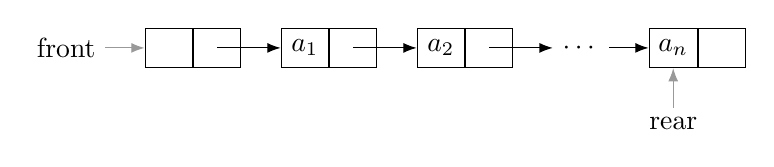
\begin{tikzpicture}[scale=0.5, box/.style={draw, minimum width=0.6cm, minimum height=0.5cm}]
    \draw node[box] (data0) {} node[box, right=0 of data0](link0){};
    \draw node[box, right=0.5 of link0] (data1) {$a_1$} node[box, right=0 of data1](link1){};
    \draw node[box, right=0.5 of link1] (data2) {$a_2$} node[box, right=0 of data2](link2){};
    \draw node[right=0.5 of link2] (more) {$\cdots$} ;
    \draw node[box, right=0.5 of more] (datan) {$a_n$} node[box, right=0 of datan](linkn){};
    \draw node[left=0.5cm of data0] (front) {front} node[below=0.5 of datan] (rear) {rear};

    \path[] (link0.center)  edge[draw, -Latex] node{}  (data1)
    (link1.center)  edge[draw, -Latex] node{}  (data2)
    (link2.center)  edge[draw, -Latex] node{}  (more)
    (more)  edge[draw, -Latex] node{}  (datan)
    (front) edge[draw=black!40, -Latex] (data0)
    (rear) edge[draw=black!40, -Latex] (datan);
  \end{tikzpicture}
\end{center}


  \begin{easylist}
    & 带头结点吗?
    & 尾指针rear指向队尾元素,提高插入操作效率
    & 请写出链队的类型定义
  \end{easylist}

  \begin{minted}{java}
    class QNode{
      ElemType  data;
      QNode next;
    }
    class LQueue{
      Node head, rear;
    }
  \end{minted}
\end{frame}

\begin{frame}[fragile]
  \frametitle{链队的基本操作 --- 入队}
  \begin{center}
  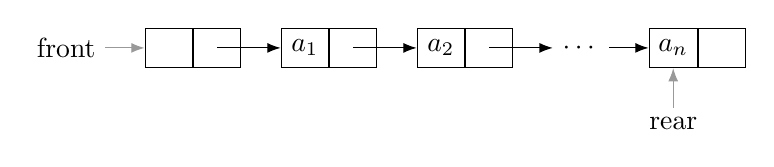
\begin{tikzpicture}[scale=0.5, box/.style={draw, minimum width=0.6cm, minimum height=0.5cm}]
    \draw node[box] (data0) {} node[box, right=0 of data0](link0){};
    \draw node[box, right=0.5 of link0] (data1) {$a_1$} node[box, right=0 of data1](link1){};
    \draw node[box, right=0.5 of link1] (data2) {$a_2$} node[box, right=0 of data2](link2){};
    \draw node[right=0.5 of link2] (more) {$\cdots$} ;
    \draw node[box, right=0.5 of more] (datan) {$a_n$} node[box, right=0 of datan](linkn){};
    \draw node[left=0.5cm of data0] (front) {front} node[below=0.5 of datan] (rear) {rear};

    \path[] (link0.center)  edge[draw, -Latex] node{}  (data1)
    (link1.center)  edge[draw, -Latex] node{}  (data2)
    (link2.center)  edge[draw, -Latex] node{}  (more)
    (more)  edge[draw, -Latex] node{}  (datan)
    (front) edge[draw=black!40, -Latex] (data0)
    (rear) edge[draw=black!40, -Latex] (datan);
  \end{tikzpicture}
\end{center}


  \begin{minted}{java}
    void InQueue(ElemType  x) {
      rear.next=new QNode(x,null);
      rear=rear.next;
    }
  \end{minted}
\end{frame}

\begin{frame}[fragile]
  \frametitle{链队的基本操作 --- 出队}
  \begin{center}
  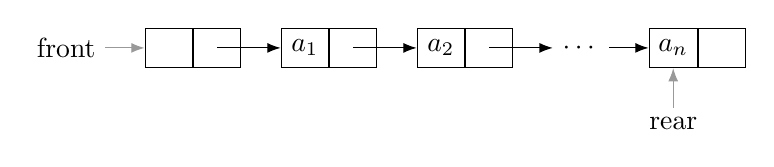
\begin{tikzpicture}[scale=0.5, box/.style={draw, minimum width=0.6cm, minimum height=0.5cm}]
    \draw node[box] (data0) {} node[box, right=0 of data0](link0){};
    \draw node[box, right=0.5 of link0] (data1) {$a_1$} node[box, right=0 of data1](link1){};
    \draw node[box, right=0.5 of link1] (data2) {$a_2$} node[box, right=0 of data2](link2){};
    \draw node[right=0.5 of link2] (more) {$\cdots$} ;
    \draw node[box, right=0.5 of more] (datan) {$a_n$} node[box, right=0 of datan](linkn){};
    \draw node[left=0.5cm of data0] (front) {front} node[below=0.5 of datan] (rear) {rear};

    \path[] (link0.center)  edge[draw, -Latex] node{}  (data1)
    (link1.center)  edge[draw, -Latex] node{}  (data2)
    (link2.center)  edge[draw, -Latex] node{}  (more)
    (more)  edge[draw, -Latex] node{}  (datan)
    (front) edge[draw=black!40, -Latex] (data0)
    (rear) edge[draw=black!40, -Latex] (datan);
  \end{tikzpicture}
\end{center}


  \begin{minted}{java}
    ElemType OutQueue() {
      QNode p;
      if (front==rear) {
        printf ("队空");
        return null;
      } else {
        p=front.next;    //把队的第一个结点取出
        front.next=p.next;   //把队头直接指向原第二个结点
        e=p.data;       /*队头元素放e中*/
        if (front.next==NULL)
          rear=front;  //若只有一个元素,出队后队空,需修改队尾指针
        return e;
      }
    }
  \end{minted}
\end{frame}


\subsection{队列应用}

\begin{frame}[fragile]
  \frametitle{队列应用 --- 迷宫寻路}
  \begin{columns}
    \begin{column}[T]{0.6\linewidth}
      \begin{easylist}
        & 从迷宫入口点(1,1)出发,向四周搜索,记下所有一步能到达的坐标点;然后
        依次再从这些点出发,再记下所有一步能到达的坐标点,…,依此类推,直到到达
        迷宫的出口点(8,8)为止,然后从出口点沿搜索路径回溯直至入口。这样就找到了
        一条迷宫的最短路径,否则迷宫无路径。

        & 与基于栈的迷宫求解的异同?
      \end{easylist}
    \end{column}
    \begin{column}[T]{0.4\linewidth}
      \includegraphics[width=0.8\textwidth]{figs/stack/maze.png}
    \end{column}
  \end{columns}
\end{frame}

\begin{frame}[fragile]
  \frametitle{解法图示}
  \begin{columns}
    \begin{column}[T]{0.6\linewidth}
      \scalebox{0.8}{
        \begin{forest}
          for tree={draw, rectangle, rounded corners},
          [ {(1, 1)},
            [{(1,2)} [{(2,2)} [{(3,2)}]] ]
            [{(2,1)} [{(2,2)}, fill=yellow!50]  [{(3,1)} [{(3,2), fill=yellow!50}] [{(4,1)}]]]
          ]
        \end{forest}
      }
      \begin{easylist}
        & 上述处理的实质:
        && 对可通行路径的空间的\color{red}广度优先搜索
        & 如何向前摸索?
        & 到达出口后,如何回溯?
      \end{easylist}
    \end{column}
    \begin{column}[T]{0.4\linewidth}
      \includegraphics[width=0.8\textwidth]{figs/stack/maze.png}
    \end{column}
  \end{columns}
\end{frame}

\begin{frame}[fragile]
  \frametitle{解法图示}
  \begin{columns}
    \begin{column}[T]{0.6\linewidth}
      \begin{easylist}
        & 如何向出口摸索:搜索路径的存储1

        && 在搜索过程中必须记下每一个可到达的坐标点,以便从这些点出发继续向四周搜索,
        使用 “FIFO”的队列保存已到达的点即可.

        & 如何向入口回溯:搜索路径的存储2

        && 为了能够从出口点沿搜索路径回溯直至入口,对于每一点,记下坐标点的同时,还
        要记下到达该点的前驱点或者从前驱点来的方向(8个方向之一)。
      \end{easylist}
    \end{column}
    \begin{column}[T]{0.4\linewidth}
      \includegraphics[width=0.8\textwidth]{figs/stack/maze.png}
    \end{column}
  \end{columns}
\end{frame}

% \input{queue}
%\section{字符串}
\begin{frame}[fragile]
  \frametitle{字符串}
  计算机非数值处理的对象经常是字符串数据。如文本检索、文本聚类、文本理解等。

  \begin{itemize}
  \item 串的定义及表示
  \item 串的模式匹配
  \end{itemize}
\end{frame}

\begin{frame}[fragile]
  \frametitle{串 (String)的定义}

  \begin{itemize}
  \item 串是由零个或多个任意字符组成的字符序列。它也是一种特殊的线性表,其数据元
    素仅由一个字符组成,而且它通常是作为一个整体来处理。

例:s="Renmin University",s是串名, Renmin University为串值,其中一个个的字符称
为串的元素。

  \item 请思考如何实现上述串的存储?
  \end{itemize}
\end{frame}

\begin{frame}[fragile]
  \frametitle{字符串的存储}
  \begin{itemize}
  \item 顺序存储: 用一组地址连续的存储单元存储串值中的字符序列。
  \item 链式存储: 考虑到存储密度,可以按块分配。
  \item 在C++/Java等语言中,String就是字符串。在C语言中没有string类型变量,字符串用字符数组表示。
  \end{itemize}
\end{frame}

\begin{frame}[fragile]
  \frametitle{串的模式匹配}
  \begin{itemize}
  \item 设s和t是给定的两个串,在主串s中寻找等于子串t的部分的过程称为模式匹配, t也称为模式。
  \item 如果在s中找到等于t的子串,则称匹配成功,返回t在s中的首次出现的存储位置,否则匹配失败。
  \item 例:

    s="ababcabcacbab"

    t="abcac"
  \end{itemize}
\end{frame}

\begin{frame}[fragile]
  \frametitle{简单的模式匹配}
  \begin{columns}
    \begin{column}[T]{0.5\linewidth}
      s="ababcabcacbab" \\ t="abcac"

      \begin{itemize}
      \item Brute-Force算法
      \end{itemize}
    \end{column}
    \begin{column}[T]{0.5\linewidth}
      \includegraphics[width=0.9\textwidth]{figs/string/pattern-match.png}
    \end{column}
  \end{columns}
\end{frame}

\begin{frame}[fragile]
  \frametitle{BF算法时间复杂度分析}
  \begin{itemize}
  \item 设串s长度为n,串t长度为m。匹配成功的情况下,考虑两种极端情况。
    \begin{itemize}
    \item 在最好情况下,即每趟不成功的匹配都发生在第一对字符比较时。
    \item 例如:s=“aaaaaaaaaabc”,t=“bc”,设匹配成功发生在$s_i$处。
    \item 在前面i-1趟不成功的匹配中共比较了i-1次,第i趟成功的匹配共比较了m次,所
      以总共比较了i-1+m次。
    \item 所有匹配成功的可能共有n-m+1种,设从si开始与t串匹配成功的概率为$p_i$,
      在等概率情况下$p_i=1/(n-m+1)$,因此最好情况下平均比较的次数是:
      \[\sum_{i=1}^{n-m+1} p_i \times (i-1+m) = \sum_{i=1}^{n-m+1} \dfrac{1}{n-m+1} \times (i-1+m) = \dfrac{(n+m)}{2}\]

    \item 即最好情况下的时间复杂度是$O(n+m)$
    \end{itemize}
  \end{itemize}
\end{frame}

\begin{frame}[fragile]
  \begin{itemize}
  \item 在最坏情况下,即每趟不成功的匹配都发生在t的最后一个字符。
  \item 例如:s=“aaaaaaaaaaab”,t=“aaab”,设匹配成功发生在$s_i$处.
  \item 在前面$i-1$趟匹配中共比较了$(i-1) \times m$次,第$i$趟成功的匹配共比较了
    $m$次,所以总共比较了$i \times m$次,因此最坏的情况下平均比较的次数是:
    \[\sum_{i=1}^{n-m+1} p_i \times (i \times m) = \sum_{i=1}^{n-m+1} \dfrac{1}{n-m+1} \times (i \times m) = \dfrac{m \times (n-m+2)}{2}\]
  \item 即最坏情况下的时间复杂度是$O(n×m)$
  \end{itemize}

  \begin{tcolorbox}[title=为什么BF算法时间性能低?]
    在每趟匹配不成功时存在大量回溯 (每次移动一位开始新的比较)
  \end{tcolorbox}
\end{frame}

\begin{frame}[fragile]
  \frametitle{改进算法}

  \begin{tikzpicture}[box/.style={draw, minimum width=1cm, minimum height=0.8cm}]
    \draw node[minimum width=2cm] (a0) {主串};
    \foreach \i in {1,...,7} {
      \pgfmathtruncatemacro{\x}{\i - 1};
      \draw node[box, right=0 of a\x] (a\i) {A} ;
    }

		\draw node[box, right=0 of a7] (a8) {B}  node[box, right=0 of a8] (a9) {A}  node[box, right=0 of a9] (a10) {A} ;

		\draw node[below=of a0] (b0) {子串}
		node[box, below=of a1] (b1) {A}
		node[box, below=of a2] (b2) {A}
		node[box, below=of a3] (b3) {A}
		node[box, below=of a4, fill=red!50] (b4) {B} ;

	  \draw[draw=red, very thick, <-] (a4) -- ++(0,1);
	  \draw[draw=red, very thick, <-] (b4) -- ++(0,-1);

    \path (a4) edge[draw=red, in=90, out=115, ->, dotted, thick]  (a2);
    \path (b4) edge[draw=red, in=-90, out=-115, ->, dotted, thick]  (b1);
  \end{tikzpicture}

  \begin{itemize}
  \item 改进算法的目的是在每一趟匹配过程中出现不匹配时,向右“滑动”尽可能远的一段
    距离后,继续进行比较。那么,应当滑动多远呢?这正是各个算法各显神通之处!

  \item KMP算法: 由D. E. Knuth,J. H. Morris和V. R. Pratt同时发现

    % \item Boyer-Moore算法
  \end{itemize}
\end{frame}

\begin{frame}[fragile]
  \frametitle{KMP算法}
  利用已经得到的“部分匹配”的结果将模式向右滑动


  视频讲解:\url{https://www.bilibili.com/video/BV1AY4y157yL/}

\end{frame}

%\section{Tree}


\begin{frame}[fragile]{树和二叉树}
  树型结构是结点之间有分支,并且具有层次关系的结构,类似于自然界中的树。树有很多应
  用,比如Unix等操作系统中的目录结构。
\end{frame}

\begin{frame}[fragile]
  \frametitle{例子}
\begin{forest}
 [CEO, for tree={rectangle, minimum width=2cm}, fill=red!10
    [CFO [财务人员] ]
    [CTO [工程师] ]
    [CMO [销售人员] ]
 ]
 \node at (current bounding box.south)
 [below=1ex,draw,cloud,aspect=6,cloud puffs=30]
 {\emph{Simple Company Hierarchy}};
\end{forest}
\end{frame}

\begin{frame}[fragile, plain]
  \scalebox{0.7}{
    \begin{forest}
      [学院, for tree={draw=none, rectangle, minimum width=1cm}, fill=red!10, circle
       [社会学部, grow=west [信息资源管理学院, fill=red!10] [新闻学院] [农业与农村发展学院] [社会与人口学院]
       [公共管理学院] [教育学院]]
       [$\cdots$]
       [ 人文学部,grow=east [哲学院] [文学院] [历史学院] [国学院] [艺术学院] [外国语学院] [清史研究所]]
       ]
       \node at (current bounding box.south)
       [below=1ex,draw,cloud,aspect=6,cloud puffs=30]
       {\emph{人民大学学院设置}};
    \end{forest}
  }
\end{frame}

\begin{frame}[fragile]{内容}
  \begin{easylist} \easyitem
    & 树的基本术语
    & 二叉树
    & 遍历二叉树与线索二叉树
    & 树和森林
    & 哈夫曼树
  \end{easylist}
\end{frame}

\subsection{基本术语}

\begin{frame}[fragile]
  \frametitle{树(TREE)}树(Tree)是$n(n \geq 0)$个结点的有限集$T$。 $T$为空时称为空
  树。当$n>0$时,树有且仅有一个特定的称为根(Root)的结点,其余结点可分为$m(m \geq
  0)$个互不相交的子集$T_1, T_2, \cdots, T_m$,其中每个子集又是一棵树,称为子
  树(Subtree)。
  \begin{enumerate}
  \item 各子树是互不相交的集合。
  \item 除根结点,其它结点有唯一前驱。
  \item   一个结点可以有零个或多个后继。
  \end{enumerate}

  \begin{forest}
    [R, for tree={color=white,fill=black}, fill=red!85
    [A [C] [D] [E]]
    [B [F]]
    ]
  \end{forest}
\end{frame}

\begin{frame}[fragile]
  \frametitle{判断哪些是树结构}
  \includegraphics[width=0.3\textwidth]{dot/tree-judge1.pdf} ~~~~~
  \pause
  \includegraphics[width=0.4\textwidth]{dot/tree-judge2.pdf}
\end{frame}

\begin{frame}[fragile]
  \frametitle{判断哪些是树结构}
  \includegraphics[width=0.35\textwidth]{dot/tree-judge3.pdf} ~~~~~
  \pause
  \includegraphics[width=0.4\textwidth]{dot/tree-judge4.pdf}
\end{frame}

\begin{frame}[fragile]
  \frametitle{树的表示形式}
  \includegraphics[width=0.36\textwidth]{dot/tree-represent1.pdf}  \pause
  \scalebox{0.75}{
    \begin{tikzpicture}[b/.style={fill=black!50},n/.style={minimum width=1cm}]
      \draw node[n] (a) {A} node[b, right=0 of a, minimum width=5cm, fill=red!50]{};	

      \draw node[minimum width=0.5cm, below=0.1 of a](bh){} 
      node[n, right=0 of bh] (b) {B} node[b,fill=blue!50, minimum width=4.3cm,right=0 of b]{};	

      \draw node[minimum width=2cm, below=0.2 of bh](dh){} 
      node[n, right=0 of dh] (d) {D} node[b, minimum width=3.5cm,right=0 of d]{};	

      \draw node[minimum width=3.5cm, below=0.2 of dh](ih){} 
      node[n, right=0 of ih] (i) {I} node[b, fill=green!50, minimum width=2.8cm,right=0 of i]{};	

      \draw node[minimum width=3.5cm, below=0.2 of ih](jh){} 
      node[n, right=0 of jh] (j) {J} node[b, fill=green!50, minimum width=2.8cm,right=0 of j]{};	

      \draw node[minimum width=2cm, below=1.2 of dh](eh){} 
      node[n, right=0 of eh] (e) {E} node[b, minimum width=3.5cm,right=0 of e]{};	

      \draw node[minimum width=2cm, below=1.8 of dh](fh){} 
      node[n, right=0 of fh] (f) {F} node[b, minimum width=3.5cm,right=0 of f]{};		


      \draw node[minimum width=0.5cm, below=3.2 of a](ch){} 
      node[n, right=0 of ch] (c) {C} node[b, fill=blue!50, minimum width=4.3cm,right=0 of c]{};	

      \draw node[minimum width=2cm, below=2.8 of dh](gh){} 
      node[n, right=0 of gh] (g) {G} node[b, minimum width=3.5cm,right=0 of g]{};	
      \draw node[minimum width=2cm, below=3.2 of dh](hh){} 
      node[n, right=0 of hh] (h) {H} node[b, minimum width=3.5cm,right=0 of h]{};	

      \draw node[below=0.1 of h] {凹入表表示法};
    \end{tikzpicture}
      } \pause
  \begin{columns}[t]
    \begin{column}{0.4\textwidth}
      \centering
      \vspace{0pt}
      (A(B(D(I,J),E, F),C(G,H)))
      
      广义表表示 \\
      
      \pause
    \end{column}
    \begin{column}{0.5\textwidth}
\scalebox{0.65}{
    \begin{tikzpicture}[n/.style={ellipse,draw}]
      \draw node[n, minimum width=7.8cm, minimum height=3.5cm, fill=red!5]{}
      node[n, minimum width=4.5cm, minimum height=2.5cm, xshift=-1.2cm, fill=blue!5]{}
      node[n, minimum width=2.5cm, minimum height=1.8cm, xshift=2.5cm, fill=blue!5]{}
      node[n, minimum width=2cm, minimum height=1.8cm, xshift=-2cm, fill=yellow!5]{}
      node[n, circle,xshift=-2.5cm, fill=green!5]{I}
      node[n, circle,xshift=-1.7cm, fill=green!5]{J}
      node[n, circle,xshift=-0.5cm, fill=yellow!5]{E}
      node[n, circle,xshift=0.4cm, fill=yellow!5]{F}
      node[n, circle,xshift=2cm, fill=yellow!5]{G}
      node[n, circle,xshift=3cm, fill=yellow!5]{H}
      node[yshift=1.35cm]{A}
      node[xshift=-0.8cm,yshift=0.8cm]{B}
      node[xshift=2.5cm, yshift=0.6cm]{C}
      node[xshift=-2cm,yshift=0.6cm]{D};
      \draw node[yshift=-2.2cm] {嵌套集合表示};
    \end{tikzpicture}
  }
  
    \end{column}
  \end{columns}
\end{frame}

\begin{frame}[fragile]{}
\begin{easylist} \easyitem

\end{easylist}
\end{frame}



%\section{Graph}

\begin{frame}[fragile]{Graph}
  \begin{adjustbox}{max totalsize={.9\textwidth}{.7\textheight},center}
    \tikzstyle{every node}=[circle, draw, fill=black!50,
    inner sep=0pt, minimum width=4pt]
    % Tutte's 8-cage
    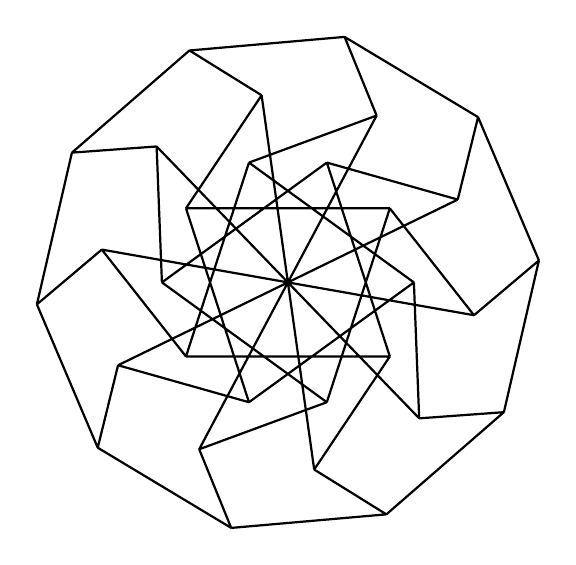
\begin{tikzpicture}[thick,scale=0.8]
      \draw \foreach \x in {0,36,...,324}
      {
        (\x:2) node {}  -- (\x+108:2)
        (\x-10:3) node {} -- (\x+5:4)
        (\x-10:3) -- (\x+36:2)
        (\x-10:3) --(\x+170:3)
        (\x+5:4) node {} -- (\x+41:4)
      };
    \end{tikzpicture}\quad

    % The largest 3-regular graph of diameter 3
    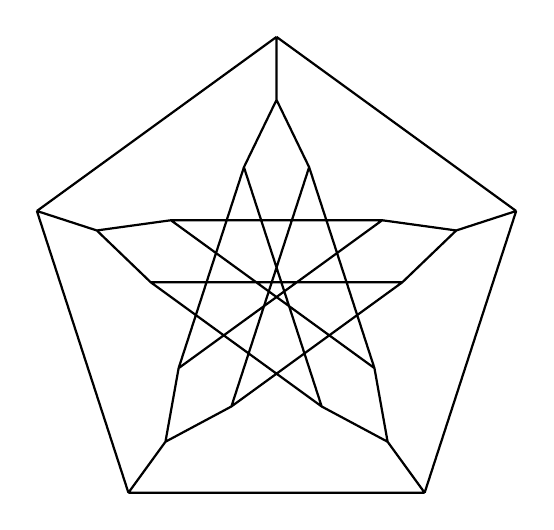
\begin{tikzpicture}[thick,scale=0.8]%
      \draw \foreach \x in {18,90,...,306} {
        (\x:4) node{} -- (\x+72:4)
        (\x:4) -- (\x:3) node{}
        (\x:3) -- (\x+15:2) node{}
        (\x:3) -- (\x-15:2) node{}
        (\x+15:2) -- (\x+144-15:2)
        (\x-15:2) -- (\x+144+15:2)
      };
    \end{tikzpicture}
  \end{adjustbox}
\end{frame}

\begin{frame}[fragile]{Content}
  \begin{easylist} \easyitem
    & 图的定义
    & 图的存储表示
    & 图的遍历
    & 图的连通性
  \end{easylist}
\end{frame}

\begin{frame}[fragile]
  \frametitle{图(Graph)}
  \begin{itemize}
  \item 图$G=(V, E)$, $V$是顶点(Vertex)集合,$E$是边/弧(Edge/Arc)的集合.
  \item 顶点的度、出度和入度
  \end{itemize}

  \begin{columns}[T]
    \column{0.5\textwidth}
    有向图:
    
    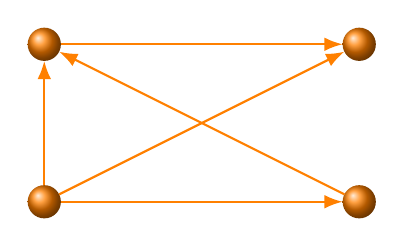
\begin{tikzpicture}[scale=1.0]
      \GraphInit[vstyle=Art]
      \Vertex{A}
      \Vertex[x=4,y=0]{B}
      \Vertex[x=0,y=2]{C}
      \Vertex[x=4,y=2]{D}
      \Edge[style={-Latex}](A)(D)

      \Edges[style={-Latex}](A,B,C, D)
      \Edges[style={-Latex}](A, C)
    \end{tikzpicture}
    
    \column{0.5\textwidth}
    无向图:
    
    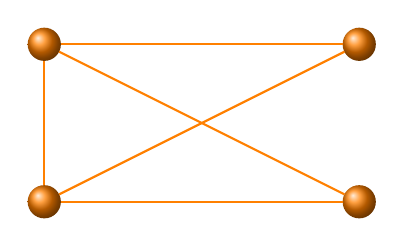
\begin{tikzpicture}[scale=1.0]
      \GraphInit[vstyle=Art]
      \Vertex{A}
      \Vertex[x=4,y=0]{B}
      \Vertex[x=0,y=2]{C}
      \Vertex[x=4,y=2]{D}
      \Edge[style={}](A)(D)

      \Edges[style={}](A,B,C, D)
      \Edges[style={}](A, C)
    \end{tikzpicture}
  \end{columns}
\end{frame}

\begin{frame}[fragile]
  \frametitle{图的相关概念}
  \includegraphics[width=0.9\textwidth]{figs/graph_concept.png}
\end{frame}

\begin{frame}[plain]
~  
\end{frame}

\begin{frame}[fragile]
  \frametitle{图的存储}
  如何表达下图的信息?
  \begin{columns}
    \column{0.4\textwidth}
    有向图:
    
    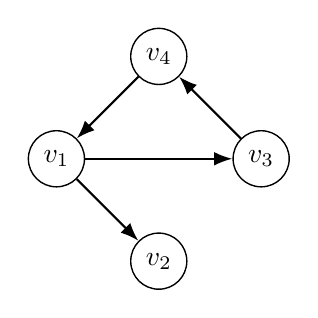
\begin{tikzpicture}[scale=1.3]
      \GraphInit[vstyle=Normal]
      \begin{scope}[rotate=180]
        \Vertices{circle}{$v_1$, $v_2$, $v_3$, $v_4$}
      \end{scope}
      \Edges[style={-Latex}]($v_1$,  $v_3$, $v_4$, $v_1$, $v_2$)
    \end{tikzpicture}
    
    \column{0.4\textwidth}
    无向图:
    
    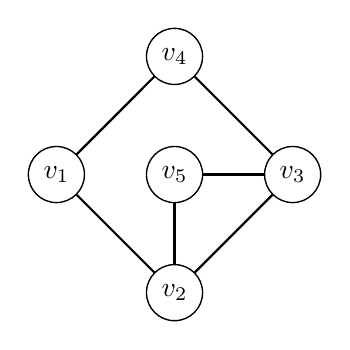
\begin{tikzpicture}[scale=1.5]
      \GraphInit[vstyle=Normal]
      \begin{scope}[rotate=180]
        \Vertices{circle}{$v_1$, $v_2$, $v_3$, $v_4$}
      \end{scope}
      \Vertex{$v_5$}
      \Edges($v_1$, $v_2$, $v_3$, $v_4$, $v_1$)
      \Edges($v_2$, $v_5$, $v_3$)
    \end{tikzpicture}
  \end{columns}
  
  \pause
  \begin{itemize}
  \item 可用邻接矩阵表达顶点及其关系。
  \end{itemize}
\end{frame}


\begin{frame}[fragile]
  \frametitle{图的存储}
  \small
  \begin{columns}[T]
    \column{0.4\textwidth}
    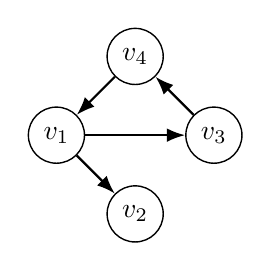
\begin{tikzpicture}[scale=1]
      \GraphInit[vstyle=Normal]
      \begin{scope}[rotate=180]
        \Vertices{circle}{$v_1$, $v_2$, $v_3$, $v_4$}
      \end{scope}
      \Edges[style={-Latex}]($v_1$,  $v_3$, $v_4$, $v_1$, $v_2$)
    \end{tikzpicture}
    \[
      \begin{blockarray}{ccccc}
         & v_1 & v_2 & v_3 & v_4 \\
        \begin{block}{c (c c c c)}
          v_1 & 0 & 1 & 1 & 0 \\
          v_2 & 0 & 0 & 0 & 0 \\
          v_3 & 0 & 0 & 0 & 1 \\
          v_4 & 1 & 0 & 0 & 0 \\
        \end{block}
      \end{blockarray}
    \]

    \column{0.4\textwidth}
    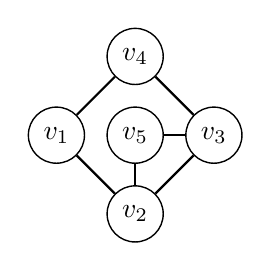
\begin{tikzpicture}[scale=1.0]
      \GraphInit[vstyle=Normal]
      \begin{scope}[rotate=180]
        \Vertices{circle}{$v_1$, $v_2$, $v_3$, $v_4$}
      \end{scope}
      \Vertex{$v_5$}
      \Edges($v_1$, $v_2$, $v_3$, $v_4$, $v_1$)
      \Edges($v_2$, $v_5$, $v_3$)
    \end{tikzpicture}

    \[
      \begin{blockarray}{cccccc}
         & v_1 & v_2 & v_3 & v_4 & v_5 \\
        \begin{block}{c (c c c c c)}
          v_1 & 0 & 1 & 0 & 1 & 0 \\
          v_2 & 1 & 0 & 1 & 0 & 1 \\
          v_3 & 0 & 1 & 0 & 1 & 1 \\
          v_4 & 1 & 0 & 1 & 0 & 0 \\
          v_5 & 0 & 1 & 1 & 0 & 0 \\
        \end{block}
      \end{blockarray}
    \]    
  \end{columns}
  
  \begin{itemize}
  \item 根据邻接矩阵,如何判断各顶点的度?
  \end{itemize}
\end{frame}

\begin{frame}[fragile]
  \frametitle{有向图的连续存储方式:邻接矩阵}
  \begin{columns}[T]
    \column{0.4\textwidth}
    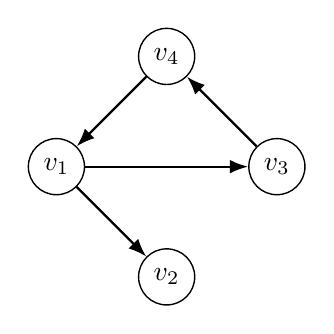
\begin{tikzpicture}[scale=1.4]
      \GraphInit[vstyle=Normal]
      \begin{scope}[rotate=180]
        \Vertices{circle}{$v_1$, $v_2$, $v_3$, $v_4$}
      \end{scope}
      \Edges[style={-Latex}]($v_1$,  $v_3$, $v_4$, $v_1$, $v_2$)
    \end{tikzpicture}
    \[
      \begin{blockarray}{ccccc}
        & v_1 & v_2 & v_3 & v_4 \\
        \begin{block}{c (c c c c)}
          v_1 & 0 & 1 & 1 & 0 \\
          v_2 & 0 & 0 & 0 & 0 \\
          v_3 & 0 & 0 & 0 & 1 \\
          v_4 & 1 & 0 & 0 & 0 \\
        \end{block}
      \end{blockarray}
    \]
    
    \column{0.6\textwidth}
    \begin{itemize}
    \item 建立二维数组$A[n][n]$, $n=|V|$
    \item 另需存放$n$个顶点信息
    \end{itemize}
  \end{columns}
\end{frame}

\begin{frame}[fragile]
  \frametitle{网的邻接矩阵}
  \begin{columns}[T]
    \column{0.4\textwidth}
    \begin{tikzpicture}[scale=1.8]
      \GraphInit[vstyle=Normal]
      \begin{scope}[rotate=180]
        \Vertices{circle}{v1, v2, v3, v4}
      \end{scope}
      \Edge[label = 8, style={-Latex}](v1)(v2)
      \Edge[label = 3, style={-Latex}](v1)(v3)
      \Edge[label = 5, style={-Latex}](v4)(v1)
      \Edge[label = 1, style={-Latex}](v3)(v4)
    \end{tikzpicture}
    \[
      \begin{blockarray}{ccccc}
        & v_1 & v_2 & v_3 & v_4 \\
        \begin{block}{c (c c c c)}
          v_1 & \infty & 8 & 3 & \infty \\
          v_2 & \infty & \infty & \infty & \infty \\
          v_3 & \infty & \infty & \infty & 1 \\
          v_4 & 5 & \infty & \infty & \infty \\
        \end{block}
      \end{blockarray}
    \]
    
    \column{0.6\textwidth}
    \begin{itemize}
    \item 有些图的边带有权重(常用来表示成本、距离、时间等), 这样的图称为:{\color{red} 网}。
    \item 网的邻接矩阵表达权重,没有边的顶点之间的权重默认为$\infty$
    \item 邻接矩阵表示方法非常直观、简单,但是会有什么问题? \pause
    \item 现实中的图经常对应稀疏矩阵,在这样情形下会有很大空间浪费.
    \end{itemize}
  \end{columns}  
\end{frame}

\begin{frame}[fragile]
  \frametitle{邻接表 (Adjacency List) -- 无向图}
  \begin{columns}[T]
    \column{0.35\textwidth}
    \begin{tikzpicture}[scale=1.3]
      \GraphInit[vstyle=Normal]
      \begin{scope}[rotate=90]
        \Vertices{circle}{v1, v2, v3, v4}
      \end{scope}
      \Edges(v3, v1, v2, v4)
    \end{tikzpicture}
    
    \column{0.6\textwidth}
    \scalebox{0.8}{
      \begin{tikzpicture}[ n/.style={minimum height=0.8cm, minimum width=1cm},
        n2/.style={minimum height=0.6cm, minimum width=1cm, fill=red!5},
        e/.style={->, very thick}]
        \draw node[n] (n0) {索引} node[n,right=0 of n0](label) {头节点};

        \foreach \x  [evaluate = \x as \xp using int(\x-1)] in {1, ..., 4}
        \draw node[n, below=0 of n\xp](n\x) {$\xp$};

        \foreach \x/\y/\z in {1/A/,2/B/,3/C/,4/D/}
        \draw node[n, right=0 of n\x, draw, fill=yellow!10](\y) {$v_\x$} node[n, right=0 of \y, draw] (P\y) {\z};


        \draw node[n2, draw, right=of PA] (c11) {2} node[n2, draw, right=0 of c11] (c12) {};
        \draw node[n2, draw, right=of c12] (c21) {1} node[n2, draw, right=0 of c21] (c22) {$\wedge$};
        \draw[e] (PA.center) -- (c11);
        \draw[e] (c12.center)--(c21);				

        \draw node[n2, draw, right=of PB] (c11) {3} node[n2, draw, right=0 of c11] (c12) {};
        \draw node[n2, draw, right=of c12] (c21) {0} node[n2, draw, right=0 of c21] (c22) {$\wedge$};
        \draw[e] (PB.center) -- (c11) (c12.center)--(c21);				

        \draw node[n2, draw, right=of PC] (c11) {0} node[n2, draw, right=0 of c11] (c12) {$\wedge$};
        \draw[e] (PC.center) -- (c11);

        \draw node[n2, draw, right=of PD] (c11) {1} node[n2, draw, right=0 of c11] (c12) {$\wedge$};
        \draw[e] (PD.center) -- (c11);
      \end{tikzpicture}
    }
  \end{columns}

  \begin{itemize}
  \item 无向图的邻接表:同一个顶点发出的边链接在同一个边链表中,便于确定顶点的度
  \item 需要$n$个头结点, $2e$个表结点
  \end{itemize}
\end{frame}

\begin{frame}[fragile]
  \frametitle{邻接表--有向图}
  \begin{columns}[T]
    \column{0.4\textwidth}
    \begin{tikzpicture}[scale=1.5]
      \GraphInit[vstyle=Normal]
      \begin{scope}[rotate=135]
        \Vertices{circle}{A, B, C, E}
      \end{scope}
      \Vertex{D}
      \Edges[style={-Latex}](A, B, C, D, E, A)
      \Edge[style={-Latex}](A)(D)	
    \end{tikzpicture}
    
    邻接表,便于确定节点出度

    \scalebox{0.7}{
      \begin{tikzpicture}[ n/.style={minimum height=0.8cm, minimum width=1cm},
        n2/.style={minimum height=0.6cm, minimum width=1cm, fill=red!5},
        e/.style={->, very thick}]
        \draw node[n] (n0) {索引} node[n,right=0 of n0](label) {头节点};

        \foreach \x  [evaluate = \x as \xp using int(\x-1)] in {1, ..., 5}
        \draw node[n, below=0 of n\xp](n\x) {$\xp$};

        \foreach \x/\y/\z in {1/A/,2/B/,3/C/,4/D/, 5/E/}
        \draw node[n, right=0 of n\x, draw, fill=yellow!10](\y) {$\y$} node[n, right=0 of \y, draw] (P\y) {\z};


        \draw node[n2, draw, right=of PA] (c11) {3} node[n2, draw, right=0 of c11] (c12) {};
        \draw node[n2, draw, right=of c12] (c21) {1} node[n2, draw, right=0 of c21] (c22) {$\wedge$};
        \draw[e] (PA.center) -- (c11);
        \draw[e] (c12.center)--(c21);				

        \draw node[n2, draw, right=of PB] (c11) {2} node[n2, draw, right=0 of c11] (c12) {$\wedge$};
        \draw[e] (PB.center) -- (c11);

        \draw node[n2, draw, right=of PC] (c11) {3} node[n2, draw, right=0 of c11] (c12) {$\wedge$};
        \draw[e] (PC.center) -- (c11);

        \draw node[n2, draw, right=of PD] (c11) {4} node[n2, draw, right=0 of c11] (c12) {$\wedge$};
        \draw[e] (PD.center) -- (c11);

        \draw node[n2, draw, right=of PE] (c11) {0} node[n2, draw, right=0 of c11] (c12) {$\wedge$};
        \draw[e] (PE.center) -- (c11);
      \end{tikzpicture}
    }
    \pause
    
    \column{0.6\textwidth}
    逆邻接表,便于确定节点入度
    
    \scalebox{0.7}{
      \begin{tikzpicture}[ n/.style={minimum height=0.8cm, minimum width=1cm},
        n2/.style={minimum height=0.6cm, minimum width=1cm, fill=red!5},
        e/.style={->, very thick}]
        \draw node[n] (n0) {索引} node[n,right=0 of n0](label) {头节点};

        \foreach \x  [evaluate = \x as \xp using int(\x-1)] in {1, ..., 5}
        \draw node[n, below=0 of n\xp](n\x) {$\xp$};

        \foreach \x/\y/\z in {1/A/,2/B/,3/C/,4/D/, 5/E/}
        \draw node[n, right=0 of n\x, draw, fill=yellow!10](\y) {$\y$} node[n, right=0 of \y, draw] (P\y) {\z};

        \draw node[n2, draw, right=of PA] (c11) {4} node[n2, draw, right=0 of c11] (c12) {$\wedge$};
        \draw[e] (PA.center) -- (c11);

        \draw node[n2, draw, right=of PB] (c11) {0} node[n2, draw, right=0 of c11] (c12) {$\wedge$};
        \draw[e] (PB.center) -- (c11);

        \draw node[n2, draw, right=of PC] (c11) {1} node[n2, draw, right=0 of c11] (c12) {$\wedge$};
        \draw[e] (PC.center) -- (c11);

        \draw node[n2, draw, right=of PD] (c11) {2} node[n2, draw, right=0 of c11] (c12) {};
        \draw node[n2, draw, right=of c12] (c21) {0} node[n2, draw, right=0 of c21] (c22) {$\wedge$};
        \draw[e] (PD.center) -- (c11);
        \draw[e] (c12.center)--(c21);		

        \draw node[n2, draw, right=of PE] (c11) {3} node[n2, draw, right=0 of c11] (c12) {$\wedge$};
        \draw[e] (PE.center) -- (c11);
      \end{tikzpicture}
    }    
  \end{columns}
\end{frame}

\begin{frame}[fragile]
  \frametitle{邻接表--权重处理}
  \scalebox{0.7}{
    \begin{tikzpicture}[scale=2]
      \GraphInit[vstyle=Normal]
      \begin{scope}[rotate=225]
        \Vertices{circle}{A, B, D, C}
      \end{scope}

      \Edge[style={-Latex}, label=1](A)(B)
      \Edge[style={-Latex, pos=0.2}, label=4](A)(D)

      \Edge[style={-Latex, pos=0.2, bend right}, label=9](B)(C)
      \Edge[style={-Latex}, label=2](B)(D)

      \Edge[style={-Latex}, label=3](C)(A)
      \Edge[style={-Latex, pos=0.2, bend right=10}, label=5](C)(B)
      \Edge[style={-Latex}, label=8](C)(D)

      \Edge[style={-Latex, bend right=40}, label=6](D)(C)
    \end{tikzpicture}
  }

  \scalebox{0.7}{
    \begin{tikzpicture}[ n/.style={minimum height=0.8cm, minimum width=1cm},
      n2/.style={minimum height=0.6cm, minimum width=1cm, fill=red!5},
      e/.style={->, very thick}]
      \draw node[n] (n0) {索引} node[n,right=0 of n0](label) {头节点};

      \foreach \x  [evaluate = \x as \xp using int(\x-1)] in {1, ..., 4}
      \draw node[n, below=0 of n\xp](n\x) {$\xp$};

      \foreach \x/\y/\z in {1/A/,2/B/,3/C/,4/D/}
      \draw node[n, right=0 of n\x, draw, fill=yellow!10](\y) {$\y$} node[n, right=0 of \y, draw] (P\y) {\z};

      \draw node[n2, draw, right=of PA] (c11) {1} node[n2, draw, right=0 of c11,fill=blue!10] (c12) {1} node[n2, draw, right=0 of c12] (c13) {};
      \draw node[n2, draw, right=of c13] (c21) {3}  node[n2, draw, right=0 of c21,fill=blue!10] (c22) {4} node[n2, draw, right=0 of c22] (c23) {$\wedge$};
      \draw[e] (PA.center) -- (c11);
      \draw[e] (c13.center) -- (c21);

      \draw node[above=of c11](tip1) {边的终点} node[right=of tip1](tip2){权重};
      \path[draw, ->] (tip1) edge (c11) (tip2) edge[bend right] (c12);
      
      \draw node[n2, draw, right=of PB] (c11) {3} node[n2, draw, right=0 of c11,fill=blue!10] (c12) {2} node[n2, draw, right=0 of c12] (c13) {};
      \draw node[n2, draw, right=of c13] (c21) {2}  node[n2, draw, right=0 of c21,fill=blue!10] (c22) {9} node[n2, draw, right=0 of c22] (c23) {$\wedge$};
      \draw[e] (PB.center) -- (c11);
      \draw[e] (c13.center) -- (c21);

      \draw node[n2, draw, right=of PC] (c11) {0} node[n2, draw, right=0 of c11,fill=blue!10] (c12) {3} node[n2, draw, right=0 of c12] (c13) {};
      \draw node[n2, draw, right=of c13] (c21) {1}  node[n2, draw, right=0 of c21,fill=blue!10] (c22) {5} node[n2, draw, right=0 of c22] (c23) {};
      \draw node[n2, draw, right=of c23] (c31) {3}  node[n2, draw, right=0 of c31,fill=blue!10] (c32) {8} node[n2, draw, right=0 of c32] (c33) {$\wedge$};
      \draw[e] (PC.center) -- (c11);
      \draw[e] (c13.center) -- (c21);
      \draw[e] (c23.center) -- (c31);

      \draw node[n2, draw, right=of PD] (c11) {2} node[n2, draw, right=0 of c11,fill=blue!10] (c12) {6} node[n2, draw, right=0 of c12] (c13) {$\wedge$};
      \draw[e] (PD.center) -- (c11);
    \end{tikzpicture}
  }
\end{frame}

\begin{frame}[fragile]
  \frametitle{练习}
  \begin{enumerate}
  \item 请写出数组存储和邻接表的类型定义
  \item 请在如下方面对比数组表示法和邻接表示法
    \begin{itemize}
    \item 存储表示是否唯一
    \item 空间复杂度
    \item 操作a: 求顶点$v_i$的度
    \item 操作b: 判定$(v_i, v_j)$是否是图的一条边
    \item 操作c: 通过遍历求边的数目
    \end{itemize}
  \end{enumerate}
\end{frame}
% TODO

\begin{frame}[fragile]
  \frametitle{比较}
  \small
  \begin{tabular}{| p{2cm} | p{4cm} | p{4cm} |}
    \hline
    ~ & 数组表示法 & 邻接表法 \\ \hline
    表示结果 & 唯一 & 不唯一 \\ \hline
    空间复杂度 & $O(n^2)$ (适用于稠密图) & $O(n+e)$ (适用于稀疏图) \\ \hline
    无向图求顶点$v_i$的度 & 第$i$行(或第$i$列)上非零元素的个数 & 第$i$个边表中的结点个数 \\ \hline
    有向图求顶点$v_i$的度  & 第$i$行上非零元素的个数是$v_i$出度,第$i$列上非零元素的个数是$v_i$的入度 & 第$i$个边表上的结点个数,求入度还需遍历各顶点的边表。逆邻接表则相反\\ \hline
    判定$(v_i, v_j)$是否是图的一条边 &  看矩阵中的$i$行$j$列是否为0 & 扫描第i个边表 \\ \hline
    求边的数目 & 检测整个矩阵中的非零元所耗费的时间是$O(N^2)$ & 对每个边表的结点个数计数所耗费的时间是$O(e+n)$ \\ \hline
  \end{tabular}  
\end{frame}

\begin{frame}[fragile]
  \frametitle{思考}

  怎么把邻接表和逆邻接表相结合,同时表示出来?
\end{frame}

\begin{frame}[fragile]
  \frametitle{有向图的十字链表}
  \begin{columns}[T]
    \column{0.4\textwidth}
    \begin{tikzpicture}[scale=1.2]
      \GraphInit[vstyle=Normal]
      \SetVertexMath
      \begin{scope}[rotate=135]
        \Vertices{circle}{A, C, D, B}
      \end{scope}
      \Edges[style={-Latex}](C,D,A,B)
      \Edges[style={-Latex}](D,B)
      \Edges[style={-Latex, bend left}](C,A,C)
    \end{tikzpicture}

    \column{0.6\textwidth}
    将邻接表、逆邻接表结合起来.
  \end{columns}
  \scalebox{0.7}{
    \begin{tikzpicture}[ n/.style={minimum height=0.8cm, minimum width=1cm},
      n2/.style={minimum height=0.6cm, minimum width=1cm, fill=red!5},
      n3/.style={minimum height=0.6cm, minimum width=1cm},
      e/.style={->, thick, red},
      e2/.style={->, thick, blue}]
      \draw node[n] (n0) {索引} node[n,right=0 of n0](label) {头节点};

      \foreach \x  [evaluate = \x as \xp using int(\x-1)] in {1, ..., 4}
      \draw node[n, below=0 of n\xp](n\x) {$\xp$};

      \foreach \x/\y/\z/\v in {1/A//,2/B//,3/C//,4/D//}
      \draw node[n, right=0 of n\x, draw, fill=yellow!10](\y) {$\y$} node[n, right=0 of \y, draw] (firstIn\y) {\z} node[n, right=0 of firstIn\y, draw] (firstOut\y) {\v};

      \draw node[n2, draw, right=of firstOutA] (headAB) {0} node[n2, draw, right=0 of headAB] (tailAB) {1} node[n3, draw, right=0 of tailAB] (headLinkAB) {} node[n3, draw, right=0 of headLinkAB] (tailLinkAB) {};

      \draw node[n2, draw, right=of tailLinkAB] (headAC) {0} node[n2, draw, right=0 of headAC] (tailAC) {2} node[n3, draw, right=0 of tailAC] (headLinkAC) {} node[n3, draw, right=0 of headLinkAC] (tailLinkAC) {$\wedge$};

      \draw node[n2, draw, right=of firstOutC] (headCA) {2} node[n2, draw, right=0 of headCA] (tailCA) {0} node[n3, draw, right=0 of tailCA] (headLinkCA) {} node[n3, draw, right=0 of headLinkCA] (tailLinkCA) {};

      \draw node[n2, draw, right=of tailLinkCA] (headCD) {2} node[n2, draw, right=0 of headCD] (tailCD) {3} node[n3, draw, right=0 of tailCD] (headLinkCD) {} node[n3, draw, right=0 of headLinkCD] (tailLinkCD) {};

      \draw node[n2, draw, right=of firstOutD] (headDA) {3} node[n2, draw, right=0 of headDA] (tailDA) {0} node[n3, draw, right=0 of tailDA] (headLinkDA) {$\wedge$} node[n3, draw, right=0 of headLinkDA] (tailLinkDA) {};

      \draw node[n2, draw, right=of tailLinkDA] (headDB) {3} node[n2, draw, right=0 of headDB] (tailDB) {1} node[n3, draw, right=0 of tailDB] (headLinkDB) {} node[n3, draw, right=0 of headLinkDB] (tailLinkDB) {};

      \draw[] node[above=1.5cm of firstInA](tipFirstIn) {$firstIn$} node[right=0 of tipFirstIn] (tipFirstOut) {$firstOut$} 
      node[above=1cm of headAB] (tipHeadAB) {$headVertex$} node[above=1.5cm of tailAB] (tipTailAB) {$tailVertex$}
      node[above=1cm of headLinkAB] (tipHeadLinkAB) {$hlink$} node[right=0 of tipHeadLinkAB] (tipTailLinkAB) {$tlink$};

      % draw tip of node
      \path[draw, <-, dashed] (tipFirstIn) edge (firstInA) 
      (tipFirstOut) edge[bend right] (firstOutA)
      (tipHeadAB) edge[] (headAB)
      (tipTailAB) edge[bend left] (tailAB)
      (tipHeadLinkAB) edge[bend left] (headLinkAB)
      (tipTailLinkAB) edge[bend left] (tailLinkAB); 

      % draw links
      \path[e] (firstInA.center) edge[bend left=45, out=120] (headLinkCA.north);
      \draw[e] (headLinkCA.center) -- (headLinkDA.north);
      \draw[e2] (firstOutA.center) -- (headAB);
      \draw[e2] (tailLinkAB.center) -- (headAC);
    \end{tikzpicture}
  }
\end{frame}

\begin{frame}[fragile]
  \frametitle{有向图的十字链表}
  \begin{minted}{java}
    class Vertex {
      String data;
      ArcBox firstIn;
      ArcBox firstOut;
    }

    class ArcBox {
      int headVertex, tailVertex;
      ArcBox hlink;
      ArcBox tlink;
      String data;
    }
  \end{minted}
\end{frame}


\begin{frame}[fragile]
  \frametitle{无向图的多重邻接表}
  \begin{tikzpicture}[scale=1.2]
    \GraphInit[vstyle=Normal]
    \SetVertexMath
    \begin{scope}[rotate=135]
      \Vertices{circle}{A, C, D, B}
    \end{scope}
    \Edges[](A, B, D, C,A,D)
  \end{tikzpicture}


  
\end{frame}
%\section{Search}


\begin{frame}[fragile]{查找表}

  \begin{center}
    \begin{matrixtable}{1.2cm}{4cm}{1.6cm}{0.6cm}{
        \head{Rank}   & \head{Distribution} & \head{Hits} & \\
        1 & Ubuntu    & 2114 & \down  \\
        2 & Fedora    & 1451 & \up    \\
        3 & Mint      & 1297 & \const \\
        4 & OpenSUSE  & 1228 & \up    \\
        5 & Debian    & 910  & \down  \\ }
    \end{matrixtable} 
  \end{center}

  查找是许多应用系统中最消耗时间的一部分,一个好的查找算法会大大提高运行速度。计
  算机需要存储包含该特定信息的表,才可以高效查找。
\end{frame}


\begin{frame}[fragile]{查找表的分类}
  \begin{easylist} \easyitem
    & 静态查找表
    && 仅作查询和检索操作的查找表。
    & 动态查找表
    && 有时在查询之后,还需要将“查询”结果为“不在查找表中”的数据元素{\em 插入}到查找表中;或者,从查找表中{\em 删除}其“查询”结果为“在查找表中”的数据元素。
  \end{easylist}
\end{frame}


\begin{frame}[fragile]{关键字}
  \begin{easylist} \easyitem
    & 是数据元素(或记录)中某个数据项的值,用以标识(识别)一个数据元素(或记录)。
    & 若此关键字可以识别唯一的一个记录,则称之谓“主关键字”。
    & 若此关键字能识别若干记录,则称之谓“次关键字”。
  \end{easylist}
\end{frame}


\begin{frame}[fragile]{查找}
  \begin{easylist} \easyitem
    & 根据给定的某个值,在查找表中确定一个其关键字等于给定值的数据元素或(记录)  
    & 若查找表中存在这样一个记录,则称“查找成功”:
    && 查找结果:给出整个记录的信息,或指示该记录在查找表中的位置;
    & 否则称“查找不成功”,查找结果:
    && 给出“空记录”或“空指针”。
  \end{easylist}
\end{frame}


\begin{frame}[fragile]{如何进行查找?}
  \begin{easylist} \easyitem
    & 查找的方法取决于查找表的结构。
    & 由于查找表中的数据元素之间不存在明显的组织规律,因此不便于查找。
    & 为了提高查找的效率, 需要在查找表中的元素之间人为地 附加某种确定的关系,换句话说, 用另外一种结构来表示查找表。
  \end{easylist}
\end{frame}


\begin{frame}[fragile]{本章大纲}
  \begin{center}
    \smartdiagram[bubble diagram]{查找表, 1. 静态查找表, 2. 动态查找表, 3. 哈希表}
  \end{center}
\end{frame}

\subsection{1. 静态查找表}
\begin{frame}[plain]
  \frametitle{}
  \centering
  \tikzstyle{mybox} = [draw=blue, fill=green!20, very thick,
  rectangle, rounded corners, inner sep=10pt, inner ysep=20pt]
  \tikzstyle{fancytitle} =[fill=blue, text=white, ellipse]
  
  \vspace{1.0cm}
  \begin{tikzpicture}[transform shape, rotate=0, baseline=-3.5cm]
    \node [mybox] (box) {%
      \begin{minipage}[t!]{0.75\textwidth}
        静态查找:对查找集合只进行查找,不涉及插入和删除操作。或者经过一段时间的查找之后,集中地进行插入和删除等修改操作。

        包括:

        \begin{itemize}
        \item 顺序查找
        \item 折半查找
        \item 分块查找
        \end{itemize}
      \end{minipage}
    };
    \node[fancytitle] at (box.north) {1. 静态查找表};
  \end{tikzpicture}
\end{frame}

\begin{frame}[fragile]
  \frametitle{顺序查找}
  \begin{easylist} \easyitem
    & 又称线性查找,是最基本的查找方法之一

    & 从表的一端向另一端逐个按给定值与关键码进行比较,若找到,查找成功,返回数据元素
    在表中的位置;若未找到与$k$相同的关键码,则返回失败信息。

    & 例:查找 $k=35$
  \end{easylist}
  
  \begin{center}
    \begin{tikzpicture}[box/.style={draw, inner sep=0.2cm, minimum size=1cm}]
      \draw[draw] node[box, fill=blue!20] (b0) {~}
      node[box, right=0 of b0] (b1) {10} 
      node[box, right=0 of b1] (b2) {15}
      node[box, right=0 of b2] (b3) {24}
      node[box, right=0 of b3] (b4) {6}
      node[box, right=0 of b4] (b5) {12}
      node[box, right=0 of b5, fill=red!10] (b6) {35}
      node[box, right=0 of b6] (b7) {40}
      node[box, right=0 of b7] (b8) {98}
      node[box, right=0 of b8] (b9) {55}; 

      \foreach \i in {0,...,9}
      {
        \draw node[above=0 of b\i] (idx_\i) {$\i$};
      };

      \path[] (b9.south) ++(0,-0.8cm) edge[-Latex, dashed] node[right]{$i$} (b9.south);
      \path[] (b6.south) ++(0,-0.8cm) edge[-Latex, very thick, draw=red] node[right]{$i$} (b6.south);

      \path[] (b8.south) ++(0,-1.2cm) edge[-Latex, very thick, draw=blue!60] node[above]{查找方向} ++(-6.5cm,0);
    \end{tikzpicture}
  \end{center}

  注意:下标为0的位置,其哨兵用途。
\end{frame}

\begin{frame}[plain]
  % Define box and box title style
  \tikzstyle{mybox} = [draw=red, fill=blue!20, very thick,
  rectangle, rounded corners, inner sep=10pt, inner ysep=20pt]
  \tikzstyle{fancytitle} =[fill=red, text=white]

  \begin{tikzpicture}
    \node [mybox] (box){%
      \begin{minipage}{0.80\textwidth}
        \begin{itemize}
        \item 分析查找算法的效率,通常用平均查找长度ASL (Average Search Length) 来衡
          量,即在查找成功时所进行的关键码比较次数的期望值。

          顺序查找(等概率情况下):

          \[
            ASL = \sum_{i=1}^{n}\dfrac{1}{n}(n-i+1) = \dfrac{n+1}{2}
          \]

          实际上,数据的查找概率存在相当大的差别!

        \item 在查找概率不同的情况下,应遵循查找表需依据查找概率越高,比较次数越少;查找概率
          越低,比较次数就较多的原则来存储数据元素。
        \end{itemize}
      \end{minipage}
    };
    \node[fancytitle, right=10pt] at (box.north west) {顺序查找的性能分析};
    % \node[fancytitle, rounded corners] at (box.east) {$\clubsuit$};
  \end{tikzpicture}
\end{frame}

\begin{frame}[fragile]
  \frametitle{顺序查找总结}
  \begin{easylist} \easyitem
    & 优点:算法简单而且使用面广。
    
    && 对表中记录的存储没有任何要求,顺序存储和链接存储均可(当然, 链式也只能用顺序
    查找);

    && 对表中记录的有序性也没有要求,无论记录是否按关键码有序均可。

    & 缺点:平均查找长度较大,特别是当待查找集合中元素较多时,查找效率较低。   
  \end{easylist}
\end{frame}

\begin{frame}[fragile]
  \frametitle{(有序表)折半查找}
  \begin{easylist} \easyitem
    & 有序表是表中数据元素按关键码升序或降序排列。

    & 适用于:

    && 线性表中的记录必须按关键码有序;
    
    && 必须采用顺序存储。
  \end{easylist}
\end{frame}

\begin{frame}[fragile]
  \frametitle{请查找14}

  \scalebox{0.7}{
    \begin{tikzpicture}[box/.style={draw, inner sep=0.2cm, minimum size=1cm}]
      \draw[draw] node[box] (b0) {~}
      node[box, right=0 of b0] (b1) {7} 
      node[box, right=0 of b1] (b2) {14}
      node[box, right=0 of b2] (b3) {18}
      node[box, right=0 of b3] (b4) {21}
      node[box, right=0 of b4] (b5) {23}
      node[box, right=0 of b5] (b6) {29}
      node[box, right=0 of b6] (b7) {31}
      node[box, right=0 of b7] (b8) {35}
      node[box, right=0 of b8] (b9) {38}
      node[box, right=0 of b9] (b10) {42}
      node[box, right=0 of b10] (b11) {46}
      node[box, right=0 of b11] (b12) {49}
      node[box, right=0 of b12] (b13) {52} ; 

      \foreach \i in {0,...,13}
      {
        \draw node[above=0 of b\i] (idx_\i) {\i};
      };

      \path[] (b1.south) ++(0,-0.5cm) edge[-Latex, thick] node[below left]{$low=1$} (b1.south);
      \path[] (b13.south) ++(0,-0.5cm) edge[-Latex, thick] node[below right]{$high=13$} (b13.south);
      \path[] (b0.south) ++(-0.5cm,-1cm) edge[draw, dashed] node[above]{\textcircled{1} 设置初始区间} ++(14.5cm,0);


      \path[] (b7.south) ++(0,-1.6cm) edge[-Latex, thick] node[below]{$mid=7$} ++(0,0.5cm)  node[right, xshift=1cm]{\textcircled{2}调整到左半区};

      \path[] (b1.south) ++(0,-2.5cm) edge[-Latex, thick] node[below left]{$low=1$} ++(0,0.5cm);
      \path[] (b6.south) ++(0,-2.5cm) edge[-Latex, thick] node[below right]{$high=6$} ++(0,0.5cm);
      \path[] (b0.south) ++(-0.5cm,-3cm) edge[draw, dashed] node[above]{} ++(14.5cm,0);


      \path[] (b3.south) ++(0,-4cm) edge[-Latex, thick] node[below]{$mid=3$} ++(0,0.5cm)  node[right, xshift=1cm]{\textcircled{3}调整到左半区};

      \path[] (b1.south) ++(0,-4.8cm) edge[-Latex, thick] node[below left]{$low=1$} ++(0,0.5cm);
      \path[] (b2.south) ++(0,-4.8cm) edge[-Latex, thick] node[below right]{$high=2$} ++(0,0.5cm);
      \path[] (b0.south) ++(-0.5cm,-5.2cm) edge[draw, dashed] node[above]{} ++(14.5cm,0);


      \path[] (b1.south) ++(0,-6cm) edge[-Latex, thick] node[below]{$mid=1$} ++(0,0.5cm) node[right, xshift=1cm]{\textcircled{4}调整到右半区};

      \path[] (b2.south) ++(0,-6.8cm) edge[-Latex, thick] node[below left]{$low=2$} ++(0,0.5cm);
      \path[] (b2.south) ++(0,-6.8cm) edge[-Latex, thick] node[below right]{$high=2$} ++(0,0.5cm);
      \path[] (b0.south) ++(-0.5cm,-7.2cm) edge[draw, dashed] node[above]{} ++(14.5cm,0);

      
      \path[] (b2.south) ++(0,-8cm) edge[-Latex, thick] node[below]{$mid=2$} ++(0,0.5cm) node[right, xshift=1cm]{\textcircled{5}查找成功};
    \end{tikzpicture}
  } 
\end{frame}

\begin{frame}[fragile]
  \frametitle{课堂练习:请查找22}
  
  \scalebox{0.7}{
    \begin{tikzpicture}[box/.style={draw, inner sep=0.2cm, minimum size=1cm}]
      \draw[draw] node[box] (b0) {~}
      node[box, right=0 of b0] (b1) {7} 
      node[box, right=0 of b1] (b2) {14}
      node[box, right=0 of b2] (b3) {18}
      node[box, right=0 of b3] (b4) {21}
      node[box, right=0 of b4] (b5) {23}
      node[box, right=0 of b5] (b6) {29}
      node[box, right=0 of b6] (b7) {31}
      node[box, right=0 of b7] (b8) {35}
      node[box, right=0 of b8] (b9) {38}
      node[box, right=0 of b9] (b10) {42}
      node[box, right=0 of b10] (b11) {46}
      node[box, right=0 of b11] (b12) {49}
      node[box, right=0 of b12] (b13) {52} ; 

      \foreach \i in {0,...,13}
      {
        \draw node[above=0 of b\i] (idx_\i) {\i};
      };
    \end{tikzpicture}
  } 
\end{frame}

\begin{frame}[fragile]
  \frametitle{}
  \begin{tikzpicture}[level distance=10mm]
    \tikzstyle{every node}=[draw,circle,inner sep=3pt, minimum size=0.5cm]
    \tikzstyle{level 1}=[sibling distance=60mm,
    set style={{every node}+=[]}]
    \tikzstyle{level 2}=[sibling distance=30mm,
    set style={{every node}+=[]}]
    \tikzstyle{level 3}=[sibling distance=20mm,
    set style={{every node}+=[]}]
    \node {31}
    child {node {18}
      child {node {7}         
        child[right] {node {14}}
      }
      child {node {23}
        child {node {21}}
        child {node {29}}
      }
    }
    child {node {42}
      child {node {35}
        child[right] {node {38}}
      }
      child {node {49}
        child {node {46}}
        child {node {52}}
      }
    };
  \end{tikzpicture}

  从折半查找过程看,以表的中点为比较对象,并以中点将表分割为两个子表,对定位到的子表
  继续这种操作。所以,对表中每个数据元素的查找过程,可用二叉树来描述。
  
  \begin{easylist} \easyitem
    & 折半查找在查找成功时,所进行的关键码比较次数至多为?
    
    & 请问平均查找长度(ASL)是多少?
  \end{easylist}
\end{frame}

\begin{frame}[fragile]
  \frametitle{}

  \begin{tikzpicture}[level distance=10mm]
    \tikzstyle{every node}=[draw,circle,inner sep=3pt, minimum size=0.5cm]
    \tikzstyle{level 1}=[sibling distance=60mm,
    set style={{every node}+=[]}]
    \tikzstyle{level 2}=[sibling distance=30mm,
    set style={{every node}+=[]}]
    \tikzstyle{level 3}=[sibling distance=20mm,
    set style={{every node}+=[]}]
    \node {31}
    child {node {18}
      child {node {7}         
        child[right] {node {14}}
      }
      child {node {23}
        child {node {21}}
        child {node {29}}
      }
    }
    child {node {42}
      child {node {35}
        child[right] {node {38}}
      }
      child {node {49}
        child {node {46}}
        child {node {52}}
      }
    };
  \end{tikzpicture}

  \begin{easylist} \easyitem
    & 折半查找在查找成功时,所进行的关键码比较次数至多为?

    \[
      \lfloor log_2 n \rfloor + 1
    \]
    
    & 请问平均查找长度(ASL)是多少?

    \[
      ASL = \dfrac{1}{n}[1 \times 2^0 + 2 \times 2^1 + \cdots + k \times  2^{k-1}]
      \approx \dfrac{n+1}{n} log_2(n+1) - 1
    \]   
  \end{easylist}
\end{frame}


\begin{frame}[fragile]
  \frametitle{分块查找}
  \begin{easylist} \easyitem

    & 分块查找又称索引顺序查找,是对顺序查找的一种改进。适用于表有序或者分块有
    序(后面的子表中所有记录的关键码均大于前一个子表的最大关键码)的情形。

    & 例:对某集合按关键码值31,62,88分为三块建立的查找表及其索引表如下:
  \end{easylist}
  
  \begin{center} 
  \scalebox{0.8}{
    \begin{tikzpicture}[box/.style={draw, minimum size=0.6cm},box2/.style={draw, minimum size=0.7cm, minimum width=1cm, fill=yellow!10}]
      \draw[draw] node[box] (b1) {14} 
      node[box, right=0 of b1] (b2) {31}
      node[box, right=0 of b2] (b3) {8}
      node[box, right=0 of b3] (b4) {22}
      node[box, right=0 of b4] (b5) {18}
      node[box, right=0 of b5] (b6) {43}
      node[box, right=0 of b6] (b7) {62}
      node[box, right=0 of b7] (b8) {49}
      node[box, right=0 of b8] (b9) {35}
      node[box, right=0 of b9] (b10) {52}
      node[box, right=0 of b10] (b11) {88}
      node[box, right=0 of b11] (b12) {78}
      node[box, right=0 of b12] (b13) {70} 
      node[box, right=0 of b13] (b14) {82}
      node[above left=0.2 of b1] {查找表}; 

      \foreach \i in {1,...,14}
      {
        \draw node[below=0 of b\i] (idx_\i) {\i};
      };

      \draw[draw] node[box2, above=1.5cm of b5] (x1) {31} 
      node[box2, right=0 of x1] (x2) {62}
      node[box2, right=0 of x2] (x3) {88}
      node[box2, below=0 of x1] (y1) {1}
      node[box2, below=0 of x2] (y2) {6}
      node[box2, below=0 of x3] (y3) {11}
      node[left=of x1] {索引表}
      node[right=0.2 of x3] {关键码字段}
      node[right=0.2 of y3] {指针字段};

      \path[draw] (y1.center) edge[-Latex] (b1.north) (y2.center) edge[-Latex] (b6.north) (y3.center) edge[-Latex] (b11.north);
    \end{tikzpicture}
  }
\end{center}
 
\end{frame}

\begin{frame}[fragile]
  \frametitle{分块查找}
  \begin{easylist} \easyitem

    & 分块查找要求将查找表分成若干个子表,并对子表建立索引表,查找表的每一个子表由
    索引表中的索引项确定。
    
    & 索引项

    && 关键码字段 (存放对应子表中的最大关键码值) ;
    && 指针字段 (存放指向对应子表的指针) ,并且要求索引项按关键码字段有序。
    
    & 如何根据索引表和查找表进行查找?
  \end{easylist}
  
  \begin{center} 
  \scalebox{0.8}{
    \begin{tikzpicture}[box/.style={draw, minimum size=0.6cm},box2/.style={draw, minimum size=0.7cm, minimum width=1cm, fill=yellow!10}]
      \draw[draw] node[box] (b1) {14} 
      node[box, right=0 of b1] (b2) {31}
      node[box, right=0 of b2] (b3) {8}
      node[box, right=0 of b3] (b4) {22}
      node[box, right=0 of b4] (b5) {18}
      node[box, right=0 of b5] (b6) {43}
      node[box, right=0 of b6] (b7) {62}
      node[box, right=0 of b7] (b8) {49}
      node[box, right=0 of b8] (b9) {35}
      node[box, right=0 of b9] (b10) {52}
      node[box, right=0 of b10] (b11) {88}
      node[box, right=0 of b11] (b12) {78}
      node[box, right=0 of b12] (b13) {70} 
      node[box, right=0 of b13] (b14) {82}
      node[above left=0.2 of b1] {查找表}; 

      \foreach \i in {1,...,14}
      {
        \draw node[below=0 of b\i] (idx_\i) {\i};
      };

      \draw[draw] node[box2, above=1.5cm of b5] (x1) {31} 
      node[box2, right=0 of x1] (x2) {62}
      node[box2, right=0 of x2] (x3) {88}
      node[box2, below=0 of x1] (y1) {1}
      node[box2, below=0 of x2] (y2) {6}
      node[box2, below=0 of x3] (y3) {11}
      node[left=of x1] {索引表}
      node[right=0.2 of x3] {关键码字段}
      node[right=0.2 of y3] {指针字段};

      \path[draw] (y1.center) edge[-Latex] (b1.north) (y2.center) edge[-Latex] (b6.north) (y3.center) edge[-Latex] (b11.north);
    \end{tikzpicture}
  }
\end{center}

\end{frame}

\begin{frame}[fragile]
  \frametitle{分块查找性能分析}

  \begin{easylist}
    & 分块查找含索引表查找和子表查找。
    
    & 设$n$个数据元素的查找表分为$m$个相同大小的子表。则分块查找的平均查找长度为:

    \[
      ASL=\dfrac{m+1}{2} + \dfrac{1}{2} \cdot \dfrac{n}{m+1}
      = \dfrac{m+\dfrac{n}{m}}{2}+1
    \]

    & 可见,平均查找长度和表的总长度$n$、子表个数$m$有关。
  \end{easylist}
  \begin{center} 
  \scalebox{0.8}{
    \begin{tikzpicture}[box/.style={draw, minimum size=0.6cm},box2/.style={draw, minimum size=0.7cm, minimum width=1cm, fill=yellow!10}]
      \draw[draw] node[box] (b1) {14} 
      node[box, right=0 of b1] (b2) {31}
      node[box, right=0 of b2] (b3) {8}
      node[box, right=0 of b3] (b4) {22}
      node[box, right=0 of b4] (b5) {18}
      node[box, right=0 of b5] (b6) {43}
      node[box, right=0 of b6] (b7) {62}
      node[box, right=0 of b7] (b8) {49}
      node[box, right=0 of b8] (b9) {35}
      node[box, right=0 of b9] (b10) {52}
      node[box, right=0 of b10] (b11) {88}
      node[box, right=0 of b11] (b12) {78}
      node[box, right=0 of b12] (b13) {70} 
      node[box, right=0 of b13] (b14) {82}
      node[above left=0.2 of b1] {查找表}; 

      \foreach \i in {1,...,14}
      {
        \draw node[below=0 of b\i] (idx_\i) {\i};
      };

      \draw[draw] node[box2, above=1.5cm of b5] (x1) {31} 
      node[box2, right=0 of x1] (x2) {62}
      node[box2, right=0 of x2] (x3) {88}
      node[box2, below=0 of x1] (y1) {1}
      node[box2, below=0 of x2] (y2) {6}
      node[box2, below=0 of x3] (y3) {11}
      node[left=of x1] {索引表}
      node[right=0.2 of x3] {关键码字段}
      node[right=0.2 of y3] {指针字段};

      \path[draw] (y1.center) edge[-Latex] (b1.north) (y2.center) edge[-Latex] (b6.north) (y3.center) edge[-Latex] (b11.north);
    \end{tikzpicture}
  }
\end{center}

\end{frame}


\subsection{2. 动态查找表}
\begin{frame}[plain]
  \frametitle{}
  \centering
  \tikzstyle{mybox} = [draw=blue, fill=green!20, very thick,
  rectangle, rounded corners, inner sep=10pt, inner ysep=20pt]
  \tikzstyle{fancytitle} =[fill=blue, text=white, ellipse]
  
  \vspace{1.0cm}
  \begin{tikzpicture}[transform shape, rotate=0, baseline=-3.5cm]
    \node [mybox] (box) {%
      \begin{minipage}[t!]{0.75\textwidth}
        动态查找表的特点是,表结构本身是在查找过程中动态生成的,即对于给定的key,若
        表中存在其关键字等于key的记录,则查找成功返回,否则插入关键字等于key的记
        录。

        包括:

        \begin{itemize}
        \item 二叉排序树
        \item 平衡二叉树
        \end{itemize}
      \end{minipage}
    };
    \node[fancytitle] at (box.north) {2. 动态查找表};
  \end{tikzpicture}
\end{frame}

\begin{frame}[fragile]
  \frametitle{二叉排序树}
  \begin{columns}[T] % align columns
    \begin{column}{0.58\linewidth}
      \begin{itemize}
      \item 二叉排序树(Binary Sort Tree)或者是一棵空树;或者是具有下列性质的二叉树:

        \textcircled{1} 若左子树不空,则左子树上所有结点的值均小于根结点的值;若
        右子树不空,则右子树上所有结点的值均大于根结点的值。

        \textcircled{2} 左右子树也都是二叉排序树。

      \item 对二叉排序树进行中序遍历,可以得到一个按关键码有序的序列,因此,一个无序序列
        可通过构造二叉排序树而成为有序序列。
      \end{itemize}
    \end{column}
    \hfill
    \begin{column}{0.38\linewidth}
      \scalebox{0.7}{
        \begin{forest}
          [ 63
          [55
          [42  [10]    [45]  ]
          [58]
          ]
          [90
          [70 [67] [83]]
          [98]
          ]
          ]
        \end{forest}
      }
    \end{column}
  \end{columns}
\end{frame}

\begin{frame}[fragile]
  \frametitle{二叉排序树的查找}

  \begin{columns}[T] % align columns
    \begin{column}{0.58\linewidth}
      \begin{itemize}
      \item 若查找树为空,查找失败;否则将key与查找树的根结点比较

        \textcircled{1} 若相等,查找成功,否则,

        \textcircled{2} 如果key<根结点关键码,继续在以左子树上进行查找

        \textcircled{3} 如果key>根结点关键码,继续在以右子树上进行查找

      \item 例如在右图所示的树上查找45
      \end{itemize}
    \end{column}
    \hfill
    \begin{column}{0.38\linewidth}
      \scalebox{0.7}{
        \begin{forest}
          [ 63
          [55, edge={->, draw=red, thick}
          [42, edge={->, draw=red, thick}  [10]    [45, edge={->, draw=red, thick}]  ]
          [58]
          ]
          [90
          [70 [67] [83]]
          [98]
          ]
          ]
        \end{forest}
      }
    \end{column}
  \end{columns} 
\end{frame}

\begin{frame}[fragile]
  \frametitle{二叉排序树的查找(cont.)}

  \begin{minipage}{0.6\textwidth}
    \begin{easylist}
      & 两树的平均查找长度分别为:

      \[
        ASL_a = \dfrac{1}{6} \times [1+2+2+3+3+3] = \dfrac{14}{6}
      \]
      
      \[
        ASL_b = \dfrac{1}{6} \times [1+2+3+4+5+6] = \dfrac{21}{6}
      \]
      
      & 二叉排序树的平均查找长度和树的形态有关!最好情况是$O(log_2 n)$.
    \end{easylist}
  \end{minipage}%
  \begin{minipage}{0.36\textwidth}
    \scalebox{0.6} {
      \begin{forest}
        [12, grow=-45 [24, grow=-45 [37, grow=-45 [45, grow=-45 [53,grow=-60
        [93]]]]]]         
      \end{forest}
    }
    \scalebox{0.6}{
      \begin{forest}
        [45 [24 [12] [37]] [53,grow=-60 [93]]]
      \end{forest}
    }
  \end{minipage}
\end{frame}

\begin{frame}[fragile]
  \frametitle{二叉排序树的构建 --- 插入节点}
  \begin{minipage}{0.6\textwidth}
    \begin{itemize}
    \item 在查找不成功时,插入该key
      \begin{itemize}
      \item 新插入结点一定是作为叶子结点添加的
      \item 插入位置在查找过程中得到
      \end{itemize}
    \item 例如查找56
    \end{itemize}
  \end{minipage}%
  \begin{minipage}{0.36\textwidth}    
    \scalebox{0.6}{
      \begin{forest}
        [63 [55 [42 [10] [ 45]] [58, grow=245 [56, fill=red!50, dotted]]] [90 [70 [67] [83]] [98]]]
      \end{forest}
    }
  \end{minipage}
\end{frame}

\begin{frame}[fragile]
  \frametitle{序列: 63, 90, 70, 55, 67, 42, 98, 83, 10, 45, 58}
  \small
  \scalebox{0.65}{
    \begin{forest}
      [63]
    \end{forest}\quad
    \begin{forest}
      [63 [, missed] [90, fill=red!10]]
    \end{forest}\quad
    \begin{forest}
      [63 [, missed] [90 [70, fill=red!10] [, missed]]]
    \end{forest}\quad
    \begin{forest}
      [63 [55, fill=red!10] [90 [70] [, missed]]]
    \end{forest}\quad
    \begin{forest}
      [63 [55] [90 [70 [67,fill=red!10] [, missed]] [, missed]]]
    \end{forest}\quad
    \begin{forest}
      [63 [55 [42,fill=red!10] [, missed]] [90 [70 [67] [, missed]] [, missed]]]
    \end{forest}\quad
    \begin{forest} 
      [63 [55 [42] [, missed]] [90 [70 [67] [, missed]] [98, fill=red!10]]]
    \end{forest}
  }

  \scalebox{0.6}{
    
    \begin{forest} 
      [63 [55 [42] [, missed]] [90 [70 [67] [83, fill=red!10]] [98]]]
    \end{forest}
    \quad
    \begin{forest} 
      [63 [55 [42 [10, fill=red!10] [,missed]] [, missed]] [90 [70 [67] [83]] [98]]]
    \end{forest}
    \quad
    \begin{forest} 
      [63 [55 [42 [10] [45, fill=red!10]] [, missed]] [90 [70 [67] [83]] [98]]]
    \end{forest}
    \quad
    \begin{forest} 
      [63 [55 [42 [10] [45]] [58, fill=red!10]] [90 [70 [67] [83]] [98]]]
    \end{forest}
  }
\end{frame}

\begin{frame}[fragile]
  \frametitle{二叉排序树的删除操作}

  依次删除结点45、90,仍要使树保持二叉排序树的特性

  
\end{frame}

\begin{frame}[fragile]{}
  \begin{easylist} \easyitem

  \end{easylist}
\end{frame}



% \section{Sorting}


\begin{frame}[plain]
  \begin{outlinebox}{内部排序大纲}
    \begin{itemize}
    \item 排序的基本概念
    \item 具体排序方法
      \begin{enumerate}
      \item \color{red} 插入排序:直接插入排序
      \item 插入排序:折半插入排序
      \item 插入排序:希尔排序
        
      \item \color{blue} 交换排序:冒泡法
      \item 交换排序:快速排序
        
      \item \color{orange} 选择排序:简单选择排序
      \item 选择排序:堆排序
        
      \item \color{purple} 归并排序:二路归并
      \item \color{gray} 基数排序
      \end{enumerate}
    \end{itemize}    
  \end{outlinebox}
\end{frame}

\begin{frame}[fragile]
  \frametitle{排序}
  \begin{easylist} \easyitem

    & 对一个数据元素集合或序列重新排列成一个按数据元素某个项值有序的序列就是排
    序。

    && 例如将关键字序列:

    $52, 49, 80, 36, 14, 58, 61, 23, 97, 75$

    调整为
    
    $14, 23, 36, 49, 52, 58, 61 ,75, 80, 97$

    && 再如将:

    $<Susie,26>, <Jack,22>, <Michel,25>, <Richard,25>$

    调整为:

    $<Jack,22>,<Michel,25>, <Richard, 25>, <Susie,26>$
  \end{easylist}
\end{frame}

\begin{frame}[fragile]
  \frametitle{排序的稳定性}
  \begin{easylist} \easyitem

    & 请注意刚才第二个序列的排序结果不唯一!

    $<Susie,26>, <Jack,22>, <Michel,25>, <Richard,25>$

    \color{red} $<Jack,22>,<Michel,25>, <Richard, 25>, <Susie,26>$

    \color{blue} $<Jack,22>, <Richard, 25>, <Michel,25>, <Susie,26>$
    
    & 稳定:若存在相同的关键字,对应位置的记录在排序后仍然保持原来的顺序,则称所使用
    的排序方法是稳定的。反之称为不稳定的。

  \end{easylist}
\end{frame}

\begin{frame}[fragile]
  \frametitle{}
  \begin{sectionbox}{插入排序}
    \begin{itemize}
    \item 直接插入排序
    \item 折半插入排序
    \item 希尔排序
    \end{itemize}
  \end{sectionbox}
\end{frame}

\begin{frame}[fragile]
  \frametitle{直接插入排序}

  对于要插入的元素$R[i]$,从$R[i-1]$起向前进行顺序查找,当$R[j-1]$小于$R[i]$时停止,插
  入位置为$R[j]$。注意在顺序表中要移动元素实现元素的插入。
  
\end{frame}


\end{document}
